\begin{partbacktext}
\part{Методы и средства проектирования интеллектуальных компьютерных систем нового поколения}
\label{part_design}

\begin{SCn}
	\scnidtf{Часть 5. Компонентное проектирование интеллектуальных компьютерных систем нового поколения}
	\scnidtf{Часть 5. Компонентное проектирование баз знаний, решателей задач и интерфейсов ostis-систем}
	\scnidtf{Часть 5. Принципы, виды и структура библиотек многократно используемых компонентов ostis-систем}
	
	\scntext{аннотация}{В данной части рассматриваются методы и средства, позволяющие повысить качество и удобство проектирования современных интеллектуальных систем. Принципы, лежащие в основе компонентного проектирования баз знаний, решателей задач и интерфейсов ostis-систем. Приведена типология многократно используемых компонентов ostis-систем, а также модель библиотек многократно используемых компонентов ostis-систем.}

	\bigskip

	\begin{scnrelfromlist}{подраздел}
		\scnitem{Глава~\ref{chapter_library}~\nameref{chapter_library}}
		\scnitem{Глава~\ref{chapter_kb_design}~\nameref{chapter_kb_design}}
		\scnitem{Глава~\ref{chapter_ps_design}~\nameref{chapter_ps_design}}
		\scnitem{Глава~\ref{chapter_ui_design}~\nameref{chapter_ui_design}}
	\end{scnrelfromlist}
\end{SCn}

\section*{Введение в Часть \ref{part_design}}

Основным результатом Искусственного интеллекта являются не сами интеллектуальные системы, а мощные и эффективные технологии их разработки. Анализ современных технологий проектирования интеллектуальных компьютерных систем показывает, что наряду с весьма впечатляющими достижениями имеют место следующие серьезные проблемы:
\begin{textitemize}
	\item Высокие требования к начальной квалификации пользователей и разработчиков. Технологии Искусственного интеллекта не ориентированы на широкий круг разработчиков и пользователей интеллектуальных систем и, следовательно, не получили массового распространения.
	\item Длительные сроки разработки интеллектуальных компьютерных систем и высокий уровень трудоемкости их сопровождения и расширения.
	\item Высока степень зависимости интеллектуальных компьютерных систем и их компонентов друг от друга, отсутствие их автоматической синхронизации. Отсутствие самодостаточности систем и компонентов, способности их функционировать отдельно друг от друга без утраты целесообразности их использования.
	\item Возрастание времени решения задачи при расширении функционала решателя задач и при расширении базы знаний системы.
	\item Отсутствие методик проектирования интеллектуальных компьютерных систем. Обновление компьютерных систем часто сводится к разработке различного рода "заплаток"{}, которые устраняют не причины выявленных недостатков обновляемых компьютерных систем, а только некоторые следствия этих причин.
	\item Отсутствие инструментальных средств проектирования интеллектуальных компьютерных систем, в том числе интеллектуальных обучающих подсистем, подсистем компонентного проектирования компьютерных систем.
\end{textitemize}
Детальнее перечисленные проблемы рассматриваются в работах \scncite{Golenkov2011}, \scncite{Ivashenko2011}, \scncite{Zalivako2011}, \scncite{Koronchik2011}, \scncite{Golenkov2013} и \scncite{Golenkov2014a}.

Для устранения возникших недостатков предлагается использовать технологию, в основе которой лежат следующие принципы, описанные в работах \scncite{Golenkov2011}, \scncite{Zalivako2011}, \scncite{Zalivako2012}, \scncite{Golenkov2013}, \scncite{Davydenko2013}, \scncite{Shunkevich2013} и \scncite{Golenkov2014a}:
\begin{textitemize}
	\item Доступность. Сравнительно неподготовленный пользователь может использовать технологию Искусственного интеллекта.
	\item Полнота. Технология должна обеспечивать решение как можно большего набора задач.
	\item Модульность. Ориентация на компонентное (модульное, сборочное) проектирование интеллектуальных систем.
	\item Поэтапное эволюционное проектирование на основе быстрого прототипирования.
	\item Высокий уровень гибкости интеллектуальных систем, простота их модификации (расширяемость). Возможность свободного добавления новых компонентов самого различного вида в интеллектуальную систему. Для этого необходимо достичь максимального уровня независимости эволюции баз знаний от эволюции решателей задач и интеллектуальных интерфейсов этих систем.
	\item Полная совместимость инструментальных средств проектирования, а также инфраструктура проектирования с проектируемыми системами --- инструментальные средства строятся как интеллектуальные системы на основе тех же принципов.
	\item Включение в состав интеллектуальных систем обучающей подсистемы как для разработчиков, так и для конечных пользователей.
	\item Включение подсистем самоанализа, самотестирования, верификации, отладки и самосовершенствования в состав разрабатываемых интеллектуальных систем.
\end{textitemize}

Интеллектуальная система должна быть ориентирована не столько на разработку определенного класса систем, сколько на их постоянное совершенствование на основе указанных принципов.

В состав технологии проектирования интеллектуальных систем входят (см. \scncite{Zalivako2012}, \scncite{Davydenko2013} и \scncite{Shunkevich2013}):
\begin{textitemize}
	\item Модель интеллектуальной компьютерной системы.
	\item Библиотека многократно используемых компонентов интеллектуальных компьютерных систем.
	\item Интеллектуальная интегрированная система автоматизации коллективного проектирования интеллектуальных компьютерных систем, включая подсистемы редактирования, отладки, оценки производительности и визуализации разработанных компонентов, а также подсистему имитационного моделирования.
	\item Методика проектирования интеллектуальных компьютерных систем.
	\item Интеллектуальный пользовательский интерфейс.
	\item Обучающие подсистемы проектирования интеллектуальных компьютерных систем, включая подсистему ведения диалога с разработчиком и пользователем.
	\item Подсистема тестирования и верификации интеллектуальных компьютерных систем, включая подсистему проверки совместимости разработанной системы с другими системами.
\end{textitemize}

\end{partbacktext}

\chapter{Комплексная библиотека многократно используемых семантически совместимых компонентов ostis-систем}
\chapauthortoc{Орлов М.К.\\Шункевич Д.В.}
\label{chapter_library}

\begin{SCn}
\begin{scnrelfromlist}{автор}
	\scnitem{Орлов М.К.}
	\scnitem{Шункевич Д.В.}
	\scnitem{Ковалёв М.В.}
	\scnitem{Садовский М.Е.}
	\scnitem{Загорский А.Г.}
	\scnitem{Банцевич К.А.}
\end{scnrelfromlist}
\end{SCn}

\bigskip

\begin{SCn}
\scntext{тезис}{Всё, что можно сделать одинаково, нужно делать одинаково.}
\end{SCn}

\bigskip

\begin{SCn}
\scntext{аннотация}{Важнейшим этапом эволюции любой технологии является переход к компонентному проектированию на основе постоянно пополняемой библиотеки многократно используемых компонентов. Идея библиотеки компонентов не нова, но семантическая мощность \textbf{\textit{Библиотеки OSTIS}} значительно выше аналогов за счет того, что подавляющее большинство компонентов библиотеки -- компоненты базы знаний, представленные на унифицированном языке смыслового представления знаний (\textit{SC-коде}). Таким образом, в Библиотеке OSTIS обеспечивается высокий уровень семантической совместимости компонентов, что приводит к высокому уровню семантической совместимости \textit{ostis-систем}, использующих комплексную библиотеку многократно используемых семантически совместимых компонентов ostis-систем.}
\end{SCn}

\bigskip

\begin{SCn}
\begin{scnrelfromlist}{библиографическая ссылка}
	\scnitem{\scncite{Golenkov2011}}
	\scnitem{\scncite{Ivashenko2011}}
	\scnitem{\scncite{Lazyrkin2011}}
	\scnitem{\scncite{Zhitko2011a}}
	\scnitem{\scncite{Zalivako2011}}
	\scnitem{\scncite{Koronchik2011}}
	\scnitem{\scncite{Zhitko2011b}}
	\scnitem{\scncite{Samodumkin2011}}
	\scnitem{\scncite{Zalivako2012}}
	\scnitem{\scncite{Golenkov2013}}
	\scnitem{\scncite{Ivashenko2013}}
	\scnitem{\scncite{Davydenko2013}}
	\scnitem{\scncite{Shunkevich2013}}
	\scnitem{\scncite{Koronchik2013}}
	\scnitem{\scncite{Eliseeva2013}}
	\scnitem{\scncite{Borisov2014}}
	\scnitem{\scncite{Golenkov2014a}}
	\scnitem{\scncite{Golenkov2014b}}
	\scnitem{\scncite{Golenkov2015}}
	\scnitem{\scncite{Shunkevich2015a}}
	\scnitem{\scncite{Shunkevich2015}}
	\scnitem{\scncite{Pivovarchik2015}}
	\scnitem{\scncite{Iyengar2021}}
	\scnitem{\scncite{Ford2019}}
	\scnitem{\scncite{Wilkes1951}}
	\scnitem{\scncite{Wilkes1953}}
	\scnitem{\scncite{Volchenskova1984}}
	\scnitem{\scncite{Blahser2021}}
	\scnitem{\scncite{Fritzson2014}}
	\scnitem{\scncite{Prakash2022}}
	\scnitem{\scncite{Memduhoglu2018}}
	\scnitem{\scncite{Moskalenko2016}}
\end{scnrelfromlist}
\end{SCn}

\bigskip

\begin{SCn}
\begin{scnrelfromlist}{подраздел}
	\scnitem{\ref{ostis_library_introduction}~\nameref{ostis_library_introduction}}
	\scnitem{\ref{ostis_library_analysis}~\nameref{ostis_library_analysis}}
	\scnitem{\ref{ostis_library_section}~\nameref{ostis_library_section}}
	\scnitem{\ref{reusable_component_section}~\nameref{reusable_component_section}}
	\scnitem{\ref{ostis_library_component_manager}~\nameref{ostis_library_component_manager}}
	\scnitem{\ref{ostis_library_conclusion}~\nameref{ostis_library_conclusion}}
\end{scnrelfromlist}
\end{SCn}

\section*{Введение в Главу \ref{chapter_library}}
\label{ostis_library_introduction}

\begin{SCn}
\begin{scnrelfromlist}{ключевое понятие}
	\scnitem{компонентное проектирование интеллектуальных систем}
\end{scnrelfromlist}
\end{SCn}

\bigskip

\begin{SCn}
\begin{scnrelfromlist}{ключевое знание}
	\scnitem{Проблемы в реализации компонентного проектирования интеллектуальных систем}
	\scnitem{Требования к реализации компонентного проектирования интеллектуальных систем}
\end{scnrelfromlist}
\end{SCn}

\bigskip

Повторное использование готовых компонентов широко применяется во многих отраслях, связанных с разработкой различного рода компьютерных систем, поскольку позволяет уменьшить трудоемкость их создания и стоимость (путем минимизации количества труда за счет отсутствия необходимости разрабатывать какой-либо компонент), повысить качество создаваемых компьютерных систем и снизить профессиональные требования к разработчикам этих систем (см. \scncite{Zhitko2011a}). Таким образом, осуществляется переход от программирования компонентов или целых систем к их проектированию (дизайну, сборке) на основе готовых компонентов (см. \scncite{Zalivako2012}). Компонентное проектирование компьютерных систем предполагает подбор существующих компонентов, способных решить поставленную задачу целиком или декомпозицию задачи на подзадачи с выделением компонентов для каждой из них (см. \scncite{Borisov2014}). Проектируемые системы по предлагаемой технологии обладают высоким уровнем гибкости, их разработка осуществляется поэтапно, переходя от одной целостной версии системы к другой. При этом стартовая версия системы может быть ядром соответствующего класса систем, входящим в библиотеку многократно используемых компонентов. Технология компонентного проектирования интеллектуальных компьютерных систем включает в себя комплекс согласованных частных технологий, обеспечивающих целостное проектирование компьютерных систем. Она включает технологию компонентного проектирования баз знаний, решателей задач, пользовательских интерфейсов и другие (см. \scncite{Golenkov2015}). Главным элементом семантической технологии компонентного проектирования интеллектуальных систем является библиотека совместимых многократно используемых компонентов. Это позволяет проектировать интеллектуальные системы комбинируя уже существующие компоненты, выбирая нужные из соответствующих библиотек (см. \scncite{Zhitko2011b}). Использование готовых компонентов предполагает, что распространяемый компонент верифицирован и документирован, а возможные ошибки и ограничения устранены либо специфицированы и известны. Создание библиотеки многократно используемых компонентов не означает пересоздание всех уже существующих современных продуктов информационных технологий. Технология компонентного проектирования интеллектуальных компьютерных систем предполагает использование огромного опыта в разработке современных компьютерных систем, однако обязательным является спецификация каждого компонента (как вновь созданного, так и интегрируемого существующего) для обеспечения возможности его установки и совместимости с другими компонентами и системами. Тем не менее эффективная технология компонентного проектирования появится только тогда, когда сформируется "критическая масса"{} разработчиков прикладных систем, участвующих в пополнении библиотек многократно используемых компонентов проектируемых систем (см. \scncite{Golenkov2013}).

Проблемы реализации компонентного подхода к проектированию интеллектуальных компьютернных систем наследуют проблемы современных технологий проектирования интеллектуальных систем, а также включают следующие (см. \scncite{Shunkevich2015a}):
\begin{SCn}
\scnheader{компонентное проектирование интеллектуальных систем}
\scnrelfrom{проблемы текущего состояния}{Проблемы в реализации компонентного проектирования интеллектуальных систем}
\begin{scnindent}
	\begin{scneqtoset}
		\scnfileitem{Отсутствие классификации компонентов на различных уровнях детализации.}
		\scnfileitem{\underline{Несовместимость} компонентов, разработанных в рамках разных проектов, вследствие отсутствия унификации в принципах представления различных видов знаний в рамках одной базы знаний, и, как следствие, отсутствие унификации в принципах выделения и спецификации многократно используемых компонентов.}
		\scnfileitem{Невозможность автоматической интеграции компонентов в систему без ручного вмешательства пользователя.}
		\scnfileitem{Не проводится тестирование, верификация и анализ качества компонентов, не выделяются преимущества, недостатки, ограничения компонентов.}
		\scnfileitem{Многие компоненты используют для идентификации язык разработчика (как правило, английский), и предполагается, что все пользователи будут использовать этот же язык. Однако для многих приложений это недопустимо – понятные только разработчику идентификаторы должны быть скрыты от конечных пользователей, которые должны быть в состоянии выбрать язык для идентификаторов, которые они видят.}
		\scnfileitem{Отсутствие средств поиска компонентов, удовлетворяющих заданных критериям.}
		\scnfileitem{Автоматическое обновление компонентов приводит к рассогласованности как отдельных модулей комьютерных систем, так и самих систем между собой.}
	\end{scneqtoset}
\end{scnindent}
\end{SCn}

Компонентное проектирование интеллектуальных компьютерных систем возможно только в том случае, если отбор компонентов будет осуществляться на основе тщательного анализа качества этих компонентов. Одним из важнейших критериев такого анализа является уровень семантической совместимости анализируемых компонентов со всеми компонентами, имеющимися в текущей версии библиотеки.

Для того, чтобы решить возникшие проблемы при проектировании интеллектуальных систем и библиотек их многократно используемых компонентов, необходимо придерживаться общих принципов технологии проектирования интеллектуальных компьютерных систем, а также выполнить следующие требования:
\begin{SCn}
\scnheader{компонентное проектирование интеллектуальных систем}
\scnrelfrom{предъявляемые требования}{Требования к реализации компонентного проектирования интеллектуальных систем}
\begin{scnindent}
	\begin{scneqtoset}
		\scnfileitem{Обеспечение совместимости (интегрируемости) компонентов интеллектуальных компьютерных систем на основе унификации представления этих компонентов.}
		\scnfileitem{Чёткое разделение процесса разработки формальных описаний интеллектуальных компьютерных систем и процесса их реализации по этому описанию.}
		\scnfileitem{Чёткое разделение разработки формального описания проектируемой интеллектуальной системы от разработки различных вариантов интерпретации таких формальных описаний систем.}
		\scnfileitem{Наличие онтологии компонентного проектирования интеллектуальных компьютерных систем, включающую (1) описание методов компонентного проектирования, (2) модель библиотеки многократно используемых компонентов, (3) модель спецификации многократно используемых компонентов, (4) полную классификацию многократно используемых компонентов, (5) описание средств взаимодействия разрабатываемой интеллектуальной компьютерной системы с библиотеками многократно используемых компонентов.}
		\scnfileitem{Наличие библиотек многократно используемых компонентов интеллектуальных компьютерных систем, включающих спецификации компонентов.}
		\scnfileitem{Наличие средств взаимодействия разрабатываемой интеллектуальной компьютерной системы с библиотеками многократно используемых компонентов для установки любых видов компонентов и управления ими в создаваемой системе.}
	\end{scneqtoset}
\end{scnindent}
\end{SCn}
Более подробно указанные принципы и требования рассмотрены в работах \scncite{Zalivako2011}, \scncite{Golenkov2013} и \scncite{Golenkov2014a}.

Большинство существующих систем создано как автономные программные продукты, которые не могут быть использованы в качестве компонентов других систем. Необходимо использовать либо целую систему, либо ничего. Небольшое число систем поддерживает компонентно-ориентированную архитектуру способную интегрироваться с другими системами (рассматривается в работах \scncite{Iyengar2021}, \scncite{Ford2019}). Однако, их интеграция возможна при условии использования одинаковых технологий и только при проектировании одной командой разработчиков.

Многократная повторная разработка уже имеющихся технических решений обусловлена либо тем, что известные технические решения плохо интегрируются в разрабатываемую систему, либо тем, что эти технические решения трудно найти. Данная проблема актуальна как в целом в сфере разработки компьютерных систем, так и в сфере разработки систем, основанных на знаниях, поскольку в системах такого рода степень согласованности различных видов знаний влияет на возможность системы решать нетривиальные задачи.

На данный момент не существует комплексной библиотеки многократно используемых семантически совместимых компонентов компьютерных систем в целом, не говоря об интеллектуальных. Существуют некоторые попытки создания библиотек типовых методов и программ для традиционных компьютерных систем, однако такие библиотеки не решают вышеперечисленные проблемы.

Термин "библиотека подпрограмм"{}, одними из первых упомянули Уилкс М., Уиллер Д. и Гилл С. в качестве одной из форм организации вычислений на компьютере (рассматривается в работах \scncite{Wilkes1951}, \scncite{Wilkes1953}). Исходя из изложенного в их книге, под библиотекой понимался набор «коротких, заранее заготовленных программ для отдельных, часто встречающихся (стандартных) вычислительных операций» (см. \scncite{Volchenskova1984}). Стоит отметить, что компонентами библиотек являются не только программы, но и компоненты интерфейса и базы знаний.

К традиционным решениям относятся \textbf{пакетные менеджеры} языков программирования и операционных систем, а также отдельные системы и платформы с встроенными компонентами и средствами для сохранения создаваемых компонентов.

Компоненты библиотеки могут быть реализованы на разных языках программирования (что приводит к тому, что для каждого языка программирования разрабатываются свои библиотеки со своими решениями различных часто встречаемых ситуаций), а также могут располагаться в разных местах, что приводит к тому, что в библиотеке необходимо средство для поиска компонентов и их установки.

\section{Анализ современных библиотек многократно используемых компонентов}
\label{ostis_library_analysis}

\begin{SCn}
\begin{scnrelfromlist}{ключевое понятие}
	\scnitem{пакетный менеджер}
\end{scnrelfromlist}
\end{SCn}

\bigskip

Современные пакетные менеджеры, такие как npm, pip, poetry, maven, apt, pacman и другие имеют преимущество в том, что они способны разрешать конфликты при установке зависимых компонентов, однако они не учитывают семантику компонентов, а только лишь устанавливают компоненты по идентификатору (см. \scncite{Blahser2021}). Библиотеки таких компонентов являются только лишь хранилищем компонентов, никак не учитывающим назначение компонентов, их преимущества и недостатки, сферы применения, иерархию компонентов и другую информацию, необходимую для интеллектуализации компонентного проектирования компьютерных систем. Поиск компонентов в библиотеках компонентов, соответствующих данных пакетным менеджерам сводится к поиску по идентификатору компонента. Также существенным недостатком современного подхода является платформенная зависимость компонентов. Современные библиотеки компонентов ориентированы только на какой-то определённый язык программирования, операционную систему или платформу.

Пакетный менеджер pip является системой управления пакетами, которая используется для установки пакетов из Python Package Index, который является некоторой библиотекой таких пакетов. Зачастую pip устанавливается вместе с Python. Пакетный менеджер pip используется только для языка программирования Python. 
Он имеет множество функций для работы с пакетами:

\begin{textitemize}
	\item установка пакета;
	\item установка пакета специализированной версии;
	\item удаление пакета;
	\item переустановка пакета;
	\item отображение установленных пакетов;
	\item поиск пакетов;
	\item верификация зависимостей пакетов;
	\item создание файла конфигурации со списком установленных пакетов и их версий;
	\item установка множества пакетов из файла конфигурации;
\end{textitemize}

\begin{figure}[H]
	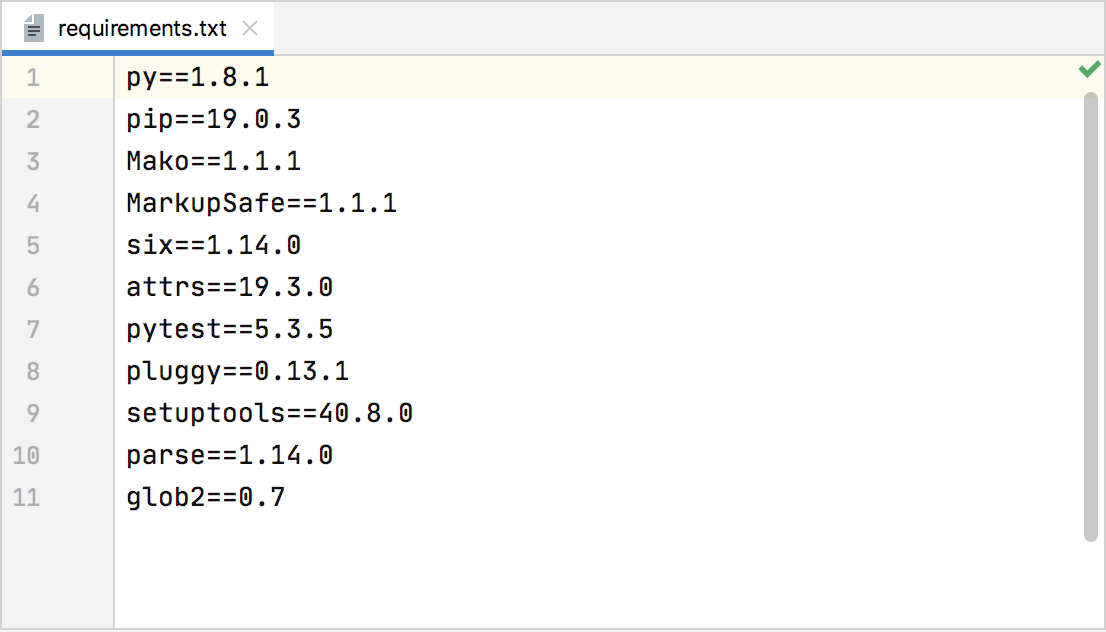
\includegraphics[scale=0.3]{author/part5/figures/pip.png}
	\caption{Файл конфигурации pip}
	\label{fig:pip}
\end{figure}

Пакетный менеджер pip хорошо работает с зависимостями, отображает безуспешно установленные пакеты, а также отображает информацию о требуемой версии пакета при конфликте с другим пакетом.

Альтернативой пакетного менеджера pip является пакетный менеджер poetry, который также ориентирован на язык программирования Python. Преимущество poetry перед pip в том, что он автоматически работает с виртуальными окружениями, способен самостоятельно их находить и создавать. Файл конфигурации для пакетов poetry является более богатым, чем у pip, он хранит такие сведения, как имя проекта, версия проекта, его описание, лицензия, список авторов, URL проекта, его документации и сайта, список ключевых слов проекта и список PyPI классификаторов. Poetry позволяет более гибко настраивать пакеты для проектов Python, файл конфигурации poetry представляет собой более богатую спецификацию проекта, однако эта спецификация не позволяет достичь совместимости между компонентами даже в рамках Python проектов и предназначена преимущественно только для чтения разработчиком. Автоматизировать проектирование компьютерных систем с помощью пакетного менеджера poetry или pip невозможно, так как требуется вмешательство разработчика, который должен вручную совместить интерфейсы устанавливаемых пакетов. Другие пакетные менеджеры языков программирования и операционных систем устроены по такому же принципу: существует хранилище компонентов (библиотека), которая представляет собой множество пакетов этого языка программирования или операционной системы и с которым взаимодействует менеджер компонентов.

\begin{figure}[H]
	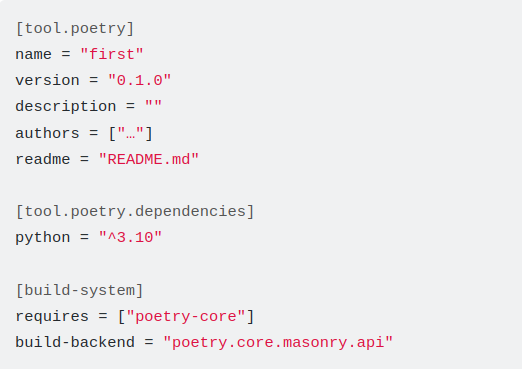
\includegraphics[scale=0.7]{author/part5/figures/poetry.png}
	\caption{Файл конфигурации poetry}
	\label{fig:poetry}
\end{figure}

В качестве компонентного подхода к проектированию программ можно рассмотреть библиотеки подпрограмм современных языков программирования, например, библиотеку стандартных шаблонов С++.

Библиотека стандартных шаблонов -- набор согласованных обобщённых алгоритмов, контейнеров, средств доступа к их содержимому и различных вспомогательных функций в C++.

В библиотеке выделяют пять основных компонентов:
\begin{textitemize}
	\item контейнер -- хранение набора объектов в памяти;
	\item итератор -- обеспечение средств доступа к содержимому контейнера;
	\item алгоритм -- определение вычислительной процедуры;
	\item адаптер -- адаптация компонентов для обеспечения различного интерфейса;
	\item функциональный объект -- сокрытие функции в объекте для использования другими компонентами.
\end{textitemize}

\begin{figure}[H]
	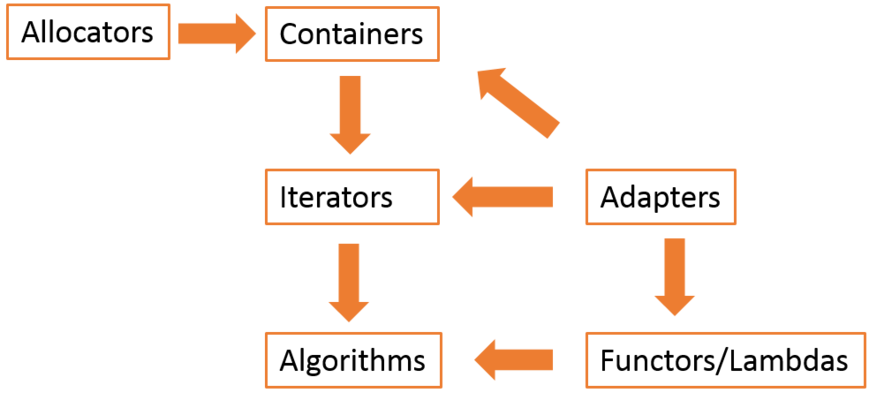
\includegraphics[scale=0.7]{author/part5/figures/STL.png}
	\caption{Структура библиотеки STL}
	\label{fig:STL}
\end{figure}

Разделение позволяет уменьшить количество компонентов. Например, вместо написания отдельной функции поиска элемента для каждого типа контейнера обеспечивается единственная версия, которая работает с каждым из них, пока соблюдаются основные требования.

Совместимость компонентов (контейнеров) в библиотеке стандартных шаблонов обеспечивается общим интерфейсом использования этих компонентов.

Компонентный подход к проектированию компьютерных систем может реализовываться в рамках различных языков, платформ и приложений. Рассмотрим некоторые из них.

Онтология, реализованная на языке OWL (Web Ontology Language), представляет собой множество декларативных утверждений о сущностях словаря предметной области (подробнее рассматривается в работе \scncite{Hepp2008}). OWL предполагает концепцию "открытого мира"{}, в соответствии с которой применимость описаний предметной области, помещённых в конкретном физическом документе, не ограничивается лишь рамками этого документа – содержание онтологии может быть использовано и дополнено другими документами, добавляющими новые факты о тех же сущностях или описывающими другую предметную область в терминах данной. "Открытость мира"{} достигается путём добавления URI каждому элементу онтологии, что позволяет воспринимать описанную на OWL онтологию как часть всеобщего объединённого знания.

На основе языка \textbf{Modelica} разработано большое число свободно доступных библиотек компонентов, одной из которых является библиотека Modelica\_StateGraph2, включающая компоненты для моделирования дискретных событий, реактивных и гибридных систем с помощью иерархических диаграмм состояния (см. \scncite{Fritzson2014}). Основным недостатком систем на базе языка Modelica является отсутствие совместимости компонентов и достаточной документации, а также узкая направленность разрабатываемых компонентов.

\textbf{Microsoft Power Apps} — это набор приложений, служб и соединителей, а также платформа данных, которая предоставляет среду разработки для эффективного создания пользовательских приложений для бизнеса. Платформа Power Apps имеет средства для создания библиотеки многократно используемых компонентов графического интерфейса, а также предварительно созданные модели распознавания текста (чтение визитных карточек или чеков) и средство обнаружение объектов, которые можно подключить к разрабатываемому приложению (см. \scncite{Prakash2022}). Библиотека компонентов Power Apps представляет собой множество создаваемых пользователем компонентов, которые можно использовать в любых приложениях. Преимущество библиотеки в том, что компоненты могут настраивать свойства по умолчанию, которые можно гибко редактировать в любых приложениях, использующих компоненты. Недостаток в том, что отсутствует семантическая совместимость компонентов, спецификация компонентов, не решена проблема существования семантически эквивалентных компонентов, нету иерархии компонентов и средств поиска этих компонентов. Компоненты платформы Microsoft Power Apps являются многократно используемыми только для однотипных приложений, которые создаются одним и тем же разработчиком.

\textbf{WebProtege} представляет собой многопользовательский веб-интерфейс, позволяющий редактировать и хранить онтологии в формате OWL в совместной среде (см. \scncite{Memduhoglu2018}). Данный проект позволяет не только создавать новые онтологии, но также загружать уже существующие онтологии, которые хранятся на сервере университета Стэнфорда. К преимуществу данного проекта можно отнести автоматическую проверку ошибок в процессе создания объектов онтологий. Данный проект является примером попытки решения проблемы накопления, систематизации и повторного использования уже существующих решений, однако, недостатком данного решения является обособленность разрабатываемых онтологий. Каждый разработанный компонент имеет свою иерархию понятий, подход к выделению классов и сущностей, которые зависят от разработчиков данных онтологий, так как в рамках данного подхода не существует универсальной модели представления знаний, а также формальной спецификации компонентов, представленных в виде онтологий. Следовательно, возникает проблема их семантической несовместимости, что, в свою очередь, приводит к невозможности повторного использования разработанных онтологий при проектировании баз знаний. Данный факт подтверждается наличием на сервере университета Стэнфорда многообразия различных онтологий на одни и те же темы.

\textbf{Платформа IACPaaS} (Intelligent Applications, Control and Platform as a Service, см. \scncite{Moskalenko2016}) – облачная платформа для разработки, управления и удаленного использования интеллектуальных облачных сервисов. Она предназначена для обеспечения поддержки разработки, управления и удаленного использования прикладных и инструментальных мультиагентных облачных сервисов (прежде всего интеллектуальных) и их компонентов для различных предметных областей. Платформа предоставляет доступ:
\begin{textitemize}
	\item прикладным пользователям (специалистам в различных предметных областях)(в качестве реализации модели SaaS) - к прикладным сервисам;
	\item разработчикам прикладных и инструментальных сервисов и их компонентов (в качестве реализации модели PaaS) - к инструментальным сервисам;
	\item управляющим интеллектуальными сервисами (в качестве реализации модели Caas);
	\item к сервисам управления.
\end{textitemize}

Платформа IACPaaS поддерживает:

\begin{textitemize}
	\item базовую технологию разработки прикладных и специализированных инструментальных (интеллектуальных) сервисов с использованием базовыхинструментальных сервисов платформы, поддерживающих эту технологию;
	\item множество специализированных технологий разработки прикладных и специализированных инструментальных (интеллектуальных) сервисов, с использованием специализированных инструментальных сервисов платформы, поддерживающих эти технологии.
\end{textitemize}

Платформа IACPaaS также не имеет средств для унифицированного представления компонентов интеллектуальных компьютерных систем и средств для их спецификации и автоматической интеграции.

Исходя из проведённого анализа можно сказать, что на текущем состоянии развития информационных технологий не существует комплексной библиотеки многократно используемых семантически совместимых компонентов компьютерных систем. Таким образом, предлагается комплексная библиотека многократно используемых семантически совместимых компонентов ostis-систем.

\section{Комплексная библиотека многократно используемых семантически совместимых компонентов ostis-систем}
\label{ostis_library_section}

\begin{SCn}
\begin{scnrelfromlist}{ключевое понятие}
	\scnitem{материнская ostis-система}
	\scnitem{библиотека многократно используемых компонентов ostis-систем}
\end{scnrelfromlist}
\end{SCn}

\bigskip

\begin{SCn}
\begin{scnrelfromlist}{ключевое знание}
	\scnitem{архитектура Экосистемы OSTIS}
\end{scnrelfromlist}
\end{SCn}

\bigskip

Основным требованием, предъявляемым к \textit{Технологии OSTIS}, является обеспечение возможности совместного использования в рамках ostis-систем различных \textit{видов знаний} и различных \textit{моделей решения задач} с возможностью \underline{неограниченного} расширения перечня используемых в ostis-системе видов знаний и моделей решения задач без существенных трудозатрат, а также различных видов интерфейсов. Следствием данного требования является необходимость реализации компонентного подхода на всех уровнях, от простых компонентов баз знаний, решателей задач и интерфейсов до целых встраиваемых ostis-систем (понятие компонента рассматривается далее в \ref{reusable_component_section}). Интеллектуальная система, спроектированная по Технологии OSTIS, представляет собой интеграцию многократно используемых компонентов баз знаний, многократно используемых компонентов решателей задач и многократно используемых компонентов интерфейсов (см. \scncite{Pivovarchik2015}). Различные многократно используемые компоненты ostis-систем объединяются в библиотеки многократно используемых компонентов ostis-систем. Разработчики \underline{любой} ostis-системы могут включить в ее состав библиотеку, которая позволит им накапливать и распространять результаты своей деятельности среди других участников \textit{Экосистемы OSTIS} в виде \textbf{\textit{многократно используемых компонентов}}. Решение о включении компонента в библиотеку принимается экспертным сообществом разработчиков, ответственным за качество этой библиотеки. Верификацию компонентов можно автоматизировать.

В рамках \textit{Экосистемы OSTIS} существует множество библиотек многократно используемых компонентов ostis-систем, являющихся подсистемами соответствующих материнских ostis-систем. Материнская ostis-система отвечает за какой-то класс компонентов и является САПРом для этого класса, содержит методики разработки таких компонентов, их классификацию, подробные пояснения ко всем подклассам компонентов. Таким образом, формируется иерархия \textbf{\textit{материнских ostis-систем}}. Материнская ostis-система в свою очередь может являться дочерней ostis-системой для какой-либо другой ostis-системы, заимствуя компоненты из библиотеки, входящей в состав этой другой ostis-системы.

\begin{SCn}
	\scnheader{ostis-система}
	\scnsuperset{материнская ostis-система}
	\begin{scnindent}
		\scnidtf{ostis-система, имеющая в своем составе библиотеку многократно используемых компонентов.}
		\scnhaselement{Метасистема OSTIS}
	\end{scnindent}
	\scnsuperset{дочерняя ostis-система}
	\begin{scnindent}
		\scnidtf{ostis-система, в составе которой имеется компонент, заимствованный из какой-либо библиотеки многократно используемых компонентов.}
	\end{scnindent}
\end{SCn}

Библиотека многократно используемых компонентов ostis-систем позволяет использовать проектный опыт по разработке и модернизации ostis-систем различного назначения.

\begin{SCn}
	\scnheader{библиотека многократно используемых компонентов ostis-систем}
	\scntext{сокращение}{библиотека компонентов ostis-систем}
	\scnidtf{комплексная библиотека многократно используемых семантически совместимых компонентов ostis-систем}
	\scnidtf{библиотека многократно используемых компонентов OSTIS}
	\scnidtf{библиотека повторно используемых компонентов OSTIS}
	\scnidtf{библиотека intelligent property компонентов ostis-систем}
	\begin{scnindent}
		\scntext{сокращение}{библиотека ip-компонентов ostis-систем}
	\end{scnindent}
	\scnhaselementrole{типичный пример}{\scnkeyword{Библиотека OSTIS}}
	\begin{scnindent}
		\scnidtf{Библиотека многократно используемых компонентов ostis-систем в составе Метасистемы OSTIS}
		\scnidtf{Библиотека Метасистемы OSTIS}
	\end{scnindent}
	\begin{scnreltoset}{объединение}
		\scnitem{библиотека многократно используемых компонентов баз знаний}
		\scnitem{библиотека многократно используемых компонентов решателей задач}
		\scnitem{библиотека многократно используемых компонентов пользовательских интерфейсов}
		\scnitem{библиотека встраиваемых ostis-систем}
		\scnitem{библиотека шаблонов типовых компонентов ostis-систем}
		\scnitem{библиотека ostis-платформ}
		\scnitem{библиотека реализаций sc-памяти}
		\scnitem{библиотека стратегий решения задач}
	\end{scnreltoset}
\end{SCn}

Главной библиотекой многократно используемых компонентов ostis-систем является \textit{Библиотека Метасистемы OSTIS}. \textit{Метасистема OSTIS} выступает \textbf{\textit{материнской системой}} для всех разрабатываемых ostis-систем, поскольку содержит все базовые компоненты (рисунок \textit{\nameref{fig:ecosystem_architecture}}).

\begin{figure}[H]
	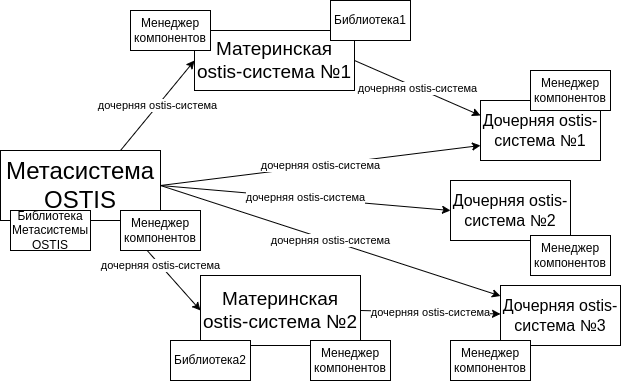
\includegraphics[scale=0.8]{author/part5/figures/ecosystem_architecture.png}
	\caption{Архитектура Экосистемы OSTIS}
	\label{fig:ecosystem_architecture}
\end{figure}

% Понятие ябиблиотеки OSTIS
Основу для реализации компонентного подхода в рамках \textit{Технологии OSTIS} составляет \textbf{\textit{Библиотека OSTIS}}. \textit{Метасистема OSTIS} ориентирована на разработку и практическое внедрение методов и средств компонентного проектирования семантически совместимых интеллектуальных систем, которая предоставляет возможность быстрого создания интеллектуальных систем различного назначения. В состав Метасистемы OSTIS входит \textbf{\textit{Библиотека OSTIS}}. Сферы практического применения технологии компонентного проектирования семантически совместимых интеллектуальных систем ничем не ограничены.

% Зачем нужна Библиотека OSTIS
Основное назначение Библиотеки OSTIS -- создание условий для эффективного, осмысленного и массового проектирования ostis-систем и их компонентов путём создания среды для накопления и совместного использования компонентов ostis-систем. Такие условия осуществляются путём неограниченного расширения постоянно эволюционируемых семантически совместимых ostis-систем и их компонентов, входящих в \textit{Экосистему OSTIS}.

Постоянно расширяемая Библиотека OSTIS существенно сокращает сроки разработки новых интеллектуальных компьютерных систем.
библиотека многократно используемых компонентов ostis-систем позволяет избавиться от дублирования семантически эквивалентных информационных компонентов. А также от многообразия форм технической реализации используемых моделей решения задач.

% Что умеет библиотека ostis-систем
Функциональные возможности библиотеки многократно используемых компонентов ostis-систем (см. \scncite{Koronchik2011}):
\begin{SCn}
	\scnheader{библиотека многократно используемых компонентов ostis-систем}
	\begin{scnrelfromset}{функциональные возможности}
		\scnfileitem{Хранение многократно используемых компонентов ostis-систем и их спецификаций. При этом часть компонентов, специфицированных в рамках библиотеки, могут физически храниться в другом месте ввиду особенностей их  технической реализации (например, исходные тексты ostis-платформы могут физически храниться в каком-либо отдельном репозитории, но специфицированы как компонент будут в соответствующей библиотеке). В этом случае спецификация компонента в рамках библиотеки должна также включать описание (1) того \underline{где} располагается компонент и (2) сценария его \underline{автоматической} установки в дочернюю ostis-систему.}
		\scnfileitem{Просмотр имеющихся компонентов и их спецификаций, а также поиск компонентов по фрагментам их спецификации.}
		\scnfileitem{Хранение сведений о статистике использования компонентов. Например, в каких ostis-системах-потребителях какие из компонентов библиотеки и какой версии используются (были скачаны). Это необходимо для учета востребованности того или иного компонента, оценки его важности и популярности.}
		\scnfileitem{Систематизация многократно используемых компонентов ostis-систем.}
		\scnfileitem{Обеспечение версионирования многократно используемых компонентов ostis-систем.}
		\scnfileitem{Поиск зависимостей между многократно используемыми компонентами в рамках библиотеки компонентов.}
		\scnfileitem{Обеспечение автоматического обновления компонентов, заимствованных в дочерние ostis-системы. Данная функция может включаться и отключаться по желанию разработчиков дочерней ostis-системы. Одновременное обновление одних и тех же компонентов во всех системах, его использующих, не должно \underline{ни в каком контексте} приводить к несогласованности между этими системами. Это требование может оказаться довольно сложным, но без него работа Экосистемы OSTIS невозможна.}
	\end{scnrelfromset}
\end{SCn}

\textit{\textbf{библиотека многократно используемых компонентов ostis-систем}} является подсистемой ostis-систем, которая имеет свою базу знаний, свой решатель задач и свой интерфейс. Однако не каждая ostis-система обязана иметь библиотеку.

\begin{SCn}
	\scnheader{библиотека многократно используемых компонентов ostis-систем}
	\begin{scnrelfromset}{обобщенная декомпозиция}
		\scnitem{база знаний библиотеки многократно используемых компонентов ostis-систем}
		\scnitem{решатель задач библиотеки многократно используемых компонентов ostis-систем}
		\scnitem{интерфейс библиотеки многократно используемых компонентов ostis-систем}
		\begin{scnindent}
			\begin{scnrelfromset}{декомпозиция}
				\scnitem{минимальный интерфейс библиотеки многократно используемых компонентов ostis-систем}
				\scnitem{расширенный интерфейс библиотеки многократно используемых компонентов ostis-систем}
				\begin{scnindent}
					\scnidtf{графический интерфейс библиотеки многократно используемых компонентов ostis-систем}
					\scnrelfrom{включение}{SCg-интерфейс библиотеки многократно используемых компонентов ostis-систем}
				\end{scnindent}
			\end{scnrelfromset}
		\end{scnindent}
	\end{scnrelfromset}
\end{SCn}

\textit{\textbf{решатель задач библиотеки многократно используемых компонентов ostis-систем}} реализует функциональные возможности библиотеки ostis-систем.

\textit{\textbf{база знаний библиотеки мнoгократно используемых компонентов ostis-систем}} представляет собой иерархию многократно используемых компонентов ostis-систем и их спецификаций.

\textit{\textbf{интерфейс библиотеки многократно используемых компонентов ostis-систем}} обеспечивает доступ к многократно используемым компонентам и возможностям библиотеки ostis-систем для пользователя и других систем (см. \scncite{Koronchik2011}). Существует минимальный и расширенный интерфейс библиотеки многократно используемых компонентов ostis-систем. Минимальный интерфейс позволяет \textit{менеджеру многократно используемых компонентов ostis-систем}, входящему в состав какой-либо дочерней ostis-системы, подключиться к библиотеке многократно используемых компонентов ostis-систем и использовать ее функциональные возможности, то есть, например, получить доступ к спецификации компонентов и установить выбранные компоненты в дочернюю ostis-систему, получить сведения до доступных версиях компонента, его зависимостях и так далее. Расширенный интерфейс, в отличие от минимального интерфейса, позволяет не только получить доступ к компонентам для дальнейшей работы с ними, но и просматривать существующую структуру библиотеки, а также компоненты и их элементы в удобном и интуитивно понятном для пользователя виде.

% Как происходит интеграция компонентов
Проблема интеграции многократно используемых компонентов ostis-систем решается путём взаимодействия компонентов через общую базу знаний. Компоненты могут лишь использовать общие ключевые узлы (понятия) в базе знаний (см. \scncite{Davydenko2013}, \scncite{Ivashenko2013} и \scncite{Golenkov2014b}). Интеграция многократно используемых компонентов ostis-систем сводится к отождествлению ключевых узлов (см. \ref{sec_ontological_formalization_basic_denotational_semantics_sc-code}) и устранению возможных дублирований и противоречий исходя из спецификации компонента и его содержания. Такой способ интеграции компонентов позволяет разрабатывать их параллельно и независимо друг от друга, что значительно сокращает сроки проектирования. Отождествление sc-элементов происходит в ходе выполнения \textit{действие. отождествить два указанных sc-элемента}, которое рассматривается в главе \ref{chapter_situation_management} Автоматическая интеграция компонентов интеллектуальных систем представляет широкие возможности для существенного сокращения сроков проектирования интеллектуальных систем, поскольку позволяет использовать опыт прошлых разработок.

Рассмотрим пример интеграции многократно используемого компонента решателя задач, который представляет собой sc-агент поиска кратчайшего пути в графе, в систему управления логистическими процессами. Допустим, система управления логистическими процессами умеет решать задачи, связанные с оптимизацией издержек в процессе создания товара и со складированием товаров. 

\begin{figure}[H]
	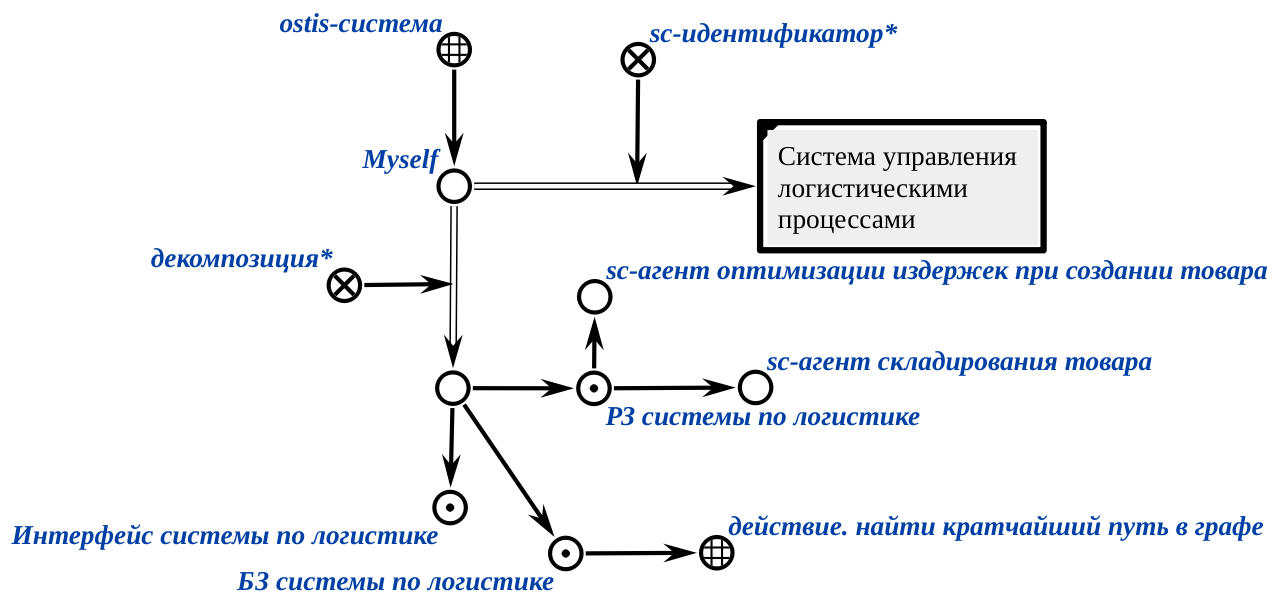
\includegraphics[scale=0.5]{author/part5/figures/logistics_system.png}
	\caption{Структура системы управления логистическими процессами}
	\label{fig:logistics_system}
\end{figure}

При этом в базе знаний системы описано, какие задачи должна решать система и соответствующие им действия. Например, действие. найти кротчайший путь в графе, которое система пока что не умеет выполнять.

Система решения задач по теории графов имеет богатую базу знаний и решатель задач, в том числе имеет sc-агент поиска кратчайшего пути в графе, который специфицирован как многократно используемый компонент и может быть использован в системе по логистике.

\begin{figure}[H]
	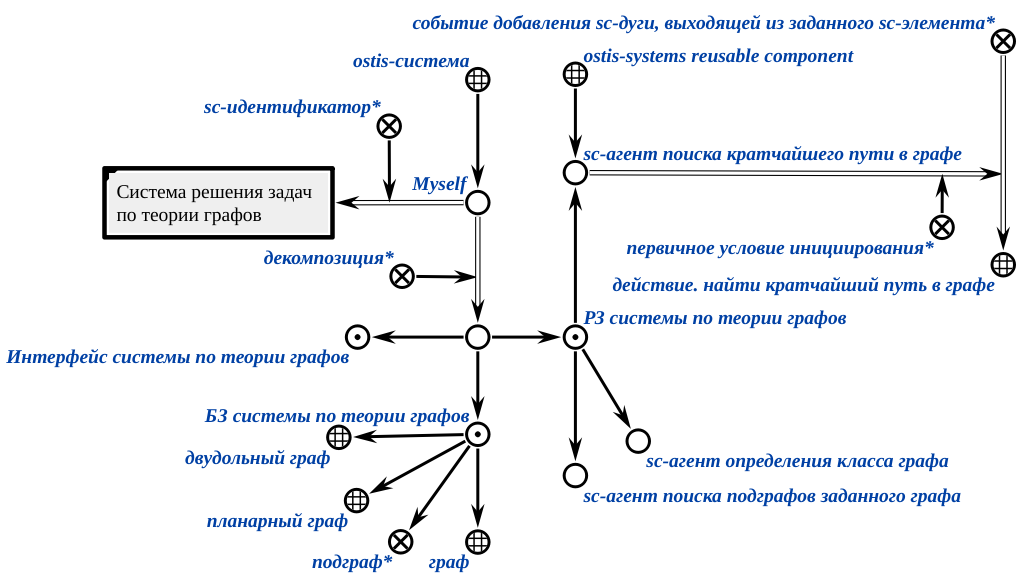
\includegraphics[scale=0.4]{author/part5/figures/graph_theory_system.png}
	\caption{Структура системы решения задач по теории графов}
	\label{fig:graph_theory_system}
\end{figure}

В результате установки многократно используемого компонента в виде sc-агента поиска кратчайшего пути в графе вся его sc-модель погружается в систему решения задач по логистике. При интеграции многократно используемого компонента, который представляет собой sc-агент поиска кратчайшего пути в графе, в систему по логистике ключевой узел \textit{действие. найти кратчайший путь в графе} системы по логистике отождествляется с таким же узлом из установленного компонента из системы по теории графов. Таким образом, при выполнении логистических задач, система сможет интерпретировать действие по поиску кратчайших путей с помощью интегрированного компонента.

% Кто ещё говорит про интеграцию фрагментов БЗ? В главе Сашеньки не рассматривается. В смысловом пространстве? 
Интеграция любых компонентов ostis-систем происходит автоматически, \underline{без} вмешательства разработчика. Это достигается за счёт использования \textit{SC-кода} и его преимуществ, унификации спецификации многократно используемых компонентов и тщательного отбора компонентов в библиотеках экспертным сообществом, ответственным за эту библиотеку.

\section{Понятие многократно используемого компонента ostis-систем}
\label{reusable_component_section}

\begin{SCn}
	\begin{scnrelfromlist}{ключевое понятие}
		\scnitem{многократно используемый компонент ostis-систем}
	\end{scnrelfromlist}
\end{SCn}

\bigskip

\begin{SCn}
	\begin{scnrelfromlist}{ключевое знание}
		\scnitem{классификация многократно используемых компонентов ostis-систем}
		\scnitem{спецификация многократно используемых компонентов ostis-систем}
	\end{scnrelfromlist}
\end{SCn}

Рассмотрим понятие многократно используемого компонента ostis-систем. Под многократно используемым компонентом ostis-систем понимается  компонент некоторой ostis-системы, который может быть использован в рамках другой ostis-системы (см. \scncite{Shunkevich2015a}). Это компонент ostis-системы, который может быть использован в других ostis-системах (\textbf{\textit{дочерних ostis-системах}}) и содержит все те и только те sc-элементы, которые необходимы для функционирования компонента в дочерней ostis-системе. Другими словами это компонент некоторой \textbf{\textit{материнской ostis-системы}}, который может быть использован в некоторой дочерней ostis-системе. Для включения многократно используемого компонента в некоторую систему, его необходимо установить в эту систему, то есть скопировать в неё все sc-элементы компонента и, при необходимости, вспомогательные файлы, такие как исходные или скомпилированные файлы компонента. Многократно используемые компоненты должны иметь унифицированную спецификацию и иерархию для поддержки \underline{совместимости} с другими компонентами. Совместимость многократно используемых компонентов приводит систему к новому качеству, к дополнительному расширению множества решаемых задач при интеграции компонентов.

\begin{SCn}
	\scnheader{многократно используемый компонент ostis-систем}
	\scnidtf{повторно используемый компонент ostis-систем}
	\scnidtf{многократно используемый компонент OSTIS}
	\scnidtf{ip-компонент ostis-систем}
	\scnidtftext{часто используемый sc-идентификатор}{многократно используемый компонент}
	\scnsubset{компонент ostis-системы}
	\scnsubset{sc-структура}
\end{SCn}

\textit{\textbf{компонент ostis-системы}} -- это целостная часть ostis-системы, которая содержит все те (и только те) sc-элементы, которые необходимы для её функционирования в ostis-системе. многократно используемый компонент ostis-систем -- это общий компонент (общая часть) для некоторого множества ostis-систем, который многократно используется, дублируется и входит в состав некоторого множества ostis-систем.
Отличие многократно используемого компонента ostis-систем от компонента ostis-системы в том, что многократно используемый компонент имеет \underline{спецификацию, достаточную для установки} этого компонента в дочернюю ostis-систему. Спецификация является частью базы знаний библиотеки многократно используемых компонентов соответствующей материнской ostis-системы. Есть техническая возможность встроить многократно используемый компонент в дочернюю ostis-систему.

Требования, предъявляемые к многократно используемым компонентам ostis-систем, наследуют общие требования к проектированию программных компонентов, а также включают следующие:
\begin{textitemize}
	\item Существует техническая возможность встроить многократно используемый компонент в дочернюю ostis-систему.
	\item Многократно используемый компонент должен выполнять свои функции наиболее общим образом, чтобы круг возможных систем, в которые он может быть встроен, был наиболее широким.
	\item Совместимость многократно используемого компонента: компонент должен стремиться повышать уровень \underline{договороспособности} ostis-систем, в которые он встроен и иметь возможность \underline{автоматической} интеграции в другие системы;
	\item Самодостаточность компонентов (или групп компонентов) технологии, то есть способности их функционировать отдельно от других компонентов без утраты целесообразности их использования.
\end{textitemize}

Рассмотрим классификацию многократно используемых компонентов ostis-систем (см. \scncite{Shunkevich2015a}). Класс многократно используемого компонента ostis-систем является важной частью спецификации компонента, позволяющей лучше понять назначение и область применения данного компонента, а также класс многократно используемого компонента является важнейшим критерием поиска компонентов в библиотеке ostis-систем. Основной признак классификации многократно используемых компонентов является признак предметной области, к которой относится компонент. Здесь структура может быть довольно богатой в соответствии с иерархией областей человеческой деятельности.

\begin{SCn}
\scnheader{многократно используемый компонент ostis-систем}
\begin{scnrelfromset}{разбиение}
	\scnitem{многократно используемый компонент базы знаний}
	\begin{scnindent}
		\scnsuperset{семантическая окрестность}
		\begin{scnindent}
			\scnhaselement{семантическая окрестность города Минска}
			\scnhaselement{семантическая окрестность понятия множество}
		\end{scnindent}
		\scnsuperset{предметная область и онтология}
		\begin{scnindent}
			\scnhaselement{предметная область и онтология треугольников}
		\end{scnindent}
		\scnsuperset{шаблон многократно используемого компонента ostis-систем}
		\begin{scnindent}
			\scnhaselement{Шаблон описания предметной области}
			\scnhaselement{Шаблон описания отношения}
		\end{scnindent}
	\end{scnindent}
	\scnitem{многократно используемый компонент решателя задач}
	\begin{scnindent}
		\scnsuperset{атомарный агент обработки знаний}
		\begin{scnindent}
			\scnhaselement{агент подсчёта мощности множества}
		\end{scnindent}
		\scnsuperset{программа обработки знаний}
		\scnsuperset{scp-машина}
		\scnsuperset{scl-машина}
	\end{scnindent}
	\scnitem{многократно используемый компонент интерфейса}
	\begin{scnindent}
		\scnsuperset{многократно используемйы компонент пользовательского интерфейса для отображения}
		\scnsuperset{интерактивный многократно используемый компонент пользовательского интерфейса}
	\end{scnindent}
\end{scnrelfromset}
\end{SCn}	

\begin{figure}[H]
	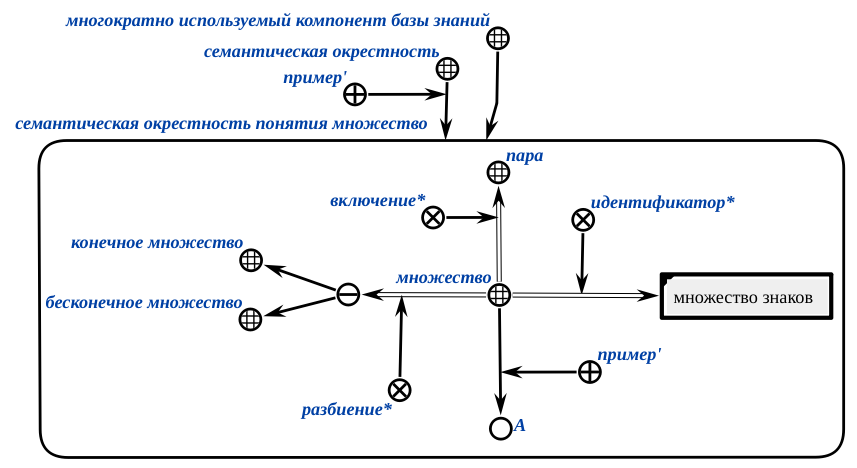
\includegraphics[scale=0.6]{author/part5/figures/set_neighbourhood.png}
	\caption{Пример многократно используемого компонента базы знаний}
	\label{fig:set_neighbourhood}
\end{figure}


Для компонентов баз знаний важнейшим признаком классификации многократно используемых компонентов является \textbf{\textit{вид используемых знаний}}. Для компонентов решателя задач -- \textbf{\textit{модель решения задач}}. Для компонентов интерфейса -- \textbf{\textit{вид интерфейса}} в соответствии с классификацией компонентов пользовательских интерфейсов.

\begin{SCn}
\scnheader{многократно используемый компонент ostis-систем}
\scnrelfrom{разбиение}{\scnkeyword{Типология компонентов ostis-систем по атомарности\scnsupergroupsign}}
\begin{scnindent}
	\begin{scneqtoset}
		\scnitem{атомарный многократно используемый компонент ostis-систем}
		\begin{scnindent}
			\scnhaselement{агент подсчёта мощности множества}
		\end{scnindent}
		\scnitem{неатомарный многократно используемый компонент ostis-систем}
		\begin{scnindent}
			\scnhaselement{агент решения геометрических задач}
		\end{scnindent}
	\end{scneqtoset}
\end{scnindent}
\end{SCn}

\textbf{\textit{атомарный многократно используемый компонент ostis-систем}} -- это компонент, который в текущем состоянии библиотеки ostis-систем рассматривается как неделимый, то есть не содержит в своем составе других компонентов. Принадлежность многократно используемого компонента ostis-систем классу атомарных компонентов зависит от того, как специфицирован этот компонент и от существующих на данный момент компонентов в библиотеке. Неатомарный многократно используемый компонент в текущем состоянии библиотеки ostis-систем содержит в своем составе другие атомарные или неатомарные компоненты, он не зависит от своих частей. Без какой-либо части неатомарного компонента его назначение сужается. В общем случае атомарный компонент может перейти в разряд неатомарных в случае, если будет принято решение выделить какую-то из его частей в качестве отдельного компонента. Все вышесказанное, однако, не означает, что даже в случае его платформенной независимости, атомарный компонент всегда хранится в sc-памяти как сформированная sc-структура. Например, платформенно-независимая реализация sc-агента всегда будет представлена набором scp-программ, но будет атомарным многократно используемым компонентом OSTIS в случае, если ни одна из этих программ не будет представлять интереса как самостоятельный компонент. В общем случае неатомарный компонент может перейти в разряд атомарных в случае, если будет принято решение по каким-либо причинам исключить все его части из рассмотрения в качестве отдельных компонентов. Следует отметить, что неатомарный компонент необязательно должен складываться \underline{полностью} из других компонентов, в его состав могут также входить и части, не являющиеся самостоятельными компонентами. Например, в состав реализованного на языке SCP sc-агента, являющего неатомарным многократно используемым компонентом могут входить как scp-программы, которые могут являться многократно используемыми компонентами (а могут и не являться), а также агентная scp-программа, которая не имеет смысла как многократно используемый компонент.

\begin{SCn}
\scnheader{многократно используемый компонент ostis-систем}
\scnrelfrom{разбиение}{\textbf{\textit{Типология компонентов ostis-систем по зависимости\scnsupergroupsign}}}
\begin{scnindent}
	\begin{scneqtoset}
		\scnitem{зависимый многократно используемый компонент ostis-систем}
		\begin{scnindent}
			\scnhaselement{визуализатор для системы по химии}
		\end{scnindent}
		\scnitem{независимый многократно используемый компонент ostis-систем}
		\begin{scnindent}
			\scnhaselement{предметная область чисел}
		\end{scnindent}
	\end{scneqtoset}
\end{scnindent}
\end{SCn}

\textbf{\textit{зависимый многократно используемый компонент ostis-систем}} зависит хотя бы от одного другого компонента библиотеки ostis-систем, то есть не может быть встроен в дочернюю ostis-систему без компонентов, от которых он зависит. независимый многократно используемый компонент ostis-систем не зависит ни от одного другого компонента библиотеки ostis-систем.

\begin{SCn}
\scnheader{многократно используемый компонент ostis-систем}
\scnrelfrom{разбиение}{\scnkeyword{Типология компонентов ostis-систем по способу их хранения\scnsupergroupsign}}
\begin{scnindent}
	\begin{scneqtoset}
		\scnitem{многократно используемый компонент ostis-систем, хранящийся в виде внешних файлов}
		\begin{scnindent}
			\begin{scnrelfromset}{разбиение}
				\scnitem{многократно используемый компонент ostis-систем, хранящийся в виде файлов исходных текстов}
				\scnitem{многократно используемый компонент ostis-систем, хранящийся в виде скомпилированных файлов}
			\end{scnrelfromset}
		\end{scnindent}
		\scnitem{многократно используемый компонент, хранящийся в виде sc-структуры}
	\end{scneqtoset}
\end{scnindent}
\end{SCn}

На данном этапе развития \textit{Технологии OSTIS} более удобным является хранение компонентов в виде исходных текстов.

\begin{SCn}
\scnheader{многократно используемый компонент ostis-систем}
\scnrelfrom{разбиение}{\scnkeyword{Типология компонентов ostis-систем по зависимости от ostis-платформы\scnsupergroupsign}}
\begin{scnindent}
	\begin{scneqtoset}
		\scnitem{платформенно-зависимый многократно используемый компонент ostis-систем}
		\begin{scnindent}
			\scnsuperset{ostis-платформа}
			\scnsuperset{абстрактный sc-агент, не реализуемый на Языке SCP}
		\end{scnindent}
		\scnitem{платформенно-независимый многократно используемый компонент ostis-систем}
		\begin{scnindent}
			\scnsuperset{многократно используемый компонент базы знаний}
			\scnsuperset{платформенно-независимый абстрактный sc-агент}
			\scnsuperset{scp-программа}
		\end{scnindent}
	\end{scneqtoset}
\end{scnindent}
\end{SCn}

Под \textbf{\textit{платформенно-зависимым многократно используемым компонентом ostis-систем}} понимается компонент, частично или полностью реализованный при помощи каких-либо сторонних с точки зрения \textit{Технологии OSTIS} средств. Недостаток таких компонентов в том, что интеграция таких компонентов в интеллектуальные системы может сопровождаться дополнительными трудностями, зависящими от конкретных средств реализации компонента. В качестве возможного преимущества платформенно-зависимых многократно используемых компонентов ostis-систем можно выделить их, как правило, более высокую производительность за счет реализации их на более приближенном к платформе уровне. В общем случае платформенно-зависимый многократно используемый компонент ostis-систем может поставляться как в виде набора исходных кодов, так и скомпилированном виде. Процесс интеграции платформенно-зависимого многократно используемого компонента ostis-систем в дочернюю систему, разработанную по Технологии OSTIS, сильно зависит от технологий реализации данного компонента и в каждом конкретном случае может состоять из различных этапов. Каждый платформенно-зависимый многократно используемый компонент ostis-систем должен иметь соответствующую подробную, корректную и понятную инструкцию по его установке и внедрению в дочернюю систему.

Под \textbf{\textit{платформенно-независимым многократно используемым компонентом ostis-систем}} понимается компонент, который целиком и полностью представлен на \textit{SC-коде}. В случае неатомарного многократно используемого компонента это означает, что все более простые компоненты, входящие в его состав также обязаны быть платформенно-независимыми многократно используемыми компонентами ostis-систем. Процесс интеграции платформенно-зависимого многократно используемого компонента ostis-систем в дочернюю систему, разработанную по Технологии OSTIS, существенно упрощается за счет использования общей унифицированной формальной основы представления и обработки знаний.

Наиболее ценными являются платформенно-независимые многократно используемые компоненты ostis-систем.

\begin{SCn}
\scnheader{многократно используемый компонент ostis-систем}
\scnrelfrom{разбиение}{\scnkeyword{Типология компонентов ostis-систем по динамичности их установки\scnsupergroupsign}}
\begin{scnindent}
	\begin{scneqtoset}
		\scnitem{динамически устанавливаемый многократно используемый компонент ostis-систем}
		\begin{scnindent}
			\scnidtf{многократно используемый компонент, при установке которого система не требует перезапуска}
			\begin{scnrelfromset}{декомпозиция}
				\scnitem{многократно используемый компонент, хранящийся в виде скомпилированных файлов}
				\scnitem{многократно используемый компонент базы знаний}
			\end{scnrelfromset}
		\end{scnindent}
		\scnitem{многократно используемый компонент, при установке которого система требует перезапуска}
	\end{scneqtoset}
\end{scnindent}
\end{SCn}


Встраиваемая ostis-система -- это неатомарный многократно используемый компонент, который состоит из базы знаний, решателя задач и интерфейса. 

\begin{SCn}
	\scnheader{встраиваемая ostis-система}
	\scnsubset{ostis-система}
	\scnsubset{неатомарный многократно используемый компонент ostis-систем}
	\begin{scnrelfromset}{декомпозиция}
		\scnitem{многократно используемый компонент базы знаний}
		\scnitem{многократно используемый компонент решателя задач}
		\scnitem{многократно используемый компонент интерфейса}
	\end{scnrelfromset}
\end{SCn}

Такими системами могут быть, например, интеллектуальный интерфейс (в том числе естественно-языковой интерфейс), среда коллективного проектирования баз знаний, менеджер многократно используемых компонентов ostis-систем, обучающая система, система тестирования и верификации интеллектуальных систем, визуальный web-ориентированный редактор sc.g-текстов и другие.

Особенность встраиваемых систем в том, что интеграция целых интеллектуальных систем предполагает интеграцию баз знаний этих систем, интеграцию их решателей задач и интеграцию их интеллектуальных интерфейсов. При интеграции встраиваемых систем база знаний встраиваемой системы становится частью базы знаний системы, в которую она встраивается, решатель задач встраиваемой системы становится частью решателя задач системы, в которую она встраивается, интерфейс встраиваемой системы становится частью интерфейса системы, в которую она встраивается. При этом встраиваемая система является целостной и может функционировать отдельно от других ostis-систем, в отличие от других многократно используемых компонентов.

Встраиваемые ostis-системы зачастую являются предметно независимыми. Таким образом, например, встраиваемая система в виде среды проектирования баз знаний может быть встроена как в систему из предметной области по геометрии, так и в систему управления аграрным объектом.

Встраиваемя ostis-система, как и любой другой многократно используемый компонент ostis-систем, должна поддерживать семантическую совместимость ostis-систем. Как сама встраиваемая ostis-система, так и все её компоненты должны быть специфицированы и согласованы. Компоненты встраиваемых ostis-систем могут быть заменены на другие, имеющие то же назначение, например, естественно-языковой интерфейс может иметь различные варианты базы знаний в зависимости от естественного языка, поддерживаемого системой, различные варианты пользовательского интерфейса, в зависимости от требований и удобства пользователей и также различные варианты реализации решателя задач для обработки естественного языка, которые могут использовать различные модели, однако решать одну и ту же задачу.

Процесс интеграции компонентов разных видов на разных этапах жизненного цикла osits-систем бывает разным. Наиболее ценными являются компоненты, которые могут быть интегрированы в работающую систему \underline{без} прекращения её функционирования. Некоторые системы, особенно системы управления, нельзя останавливать, а устанавливать и обновлять компоненты нужно.

Для того, чтобы хранить многократно используемые компоненты ostis-систем, необходимо некоторое хранилище. Таким хранилищем может выступать как какая-либо ostis-система, так и стороннее хранилище, например, облачное. Помимо внешних файлов компонента в хранилище должна находиться его \underline{спецификация}.

Каждый \textit{многократно используемый компонент ostis-систем} должен быть специфицирован в рамках библиотеки (см. \scncite{Davydenko2013}). Данные спецификации включают в себя основные знания о компоненте, которые позволяют обеспечить построение полной иерархии компонентов и их зависимостей, а также обеспечивают \underline{беспрепятственную} интеграцию компонентов в дочерние ostis-системы. Для спецификации компонента используются, как отношения, так и классы компонента.

% Параметры формализовать
Чтобы многократно используемый компонент мог быть принят в библиотеку, нужно специфицировать его, используя отношения из класса \textit{необходимое для установки отношение, специфицирующее многократно используемый компонент ostis-систем}. В то же время отношения класса \textit{необязательное для установки отношение, специфицирующее многократно используемый компонент ostis-систем} помогают лучше понять суть компонента, упрощает поиск, но не является обязательным для того, чтобы компонент мог быть установлен в ostis-систему. Спецификация многократно используемого компонента ostis-систем также включает класс (тип) компонента. Указание класса \textit{многократно используемый компонент ostis-систем} является обязательным. Сам многократно используемый компонент в рамках спецификации является \textit{ключевым sc-элементом}, а также может иметь множество своих ключевых sc-элементов. Для уточнения типа компонента могут использоваться другие классы, например дата публикации первой и последней версии компонента, качественно-количественные характеристики, какие как уровень семантической совместимости компонентов, сложность реализации компонента, уровень производительности компонента (для программ можно использовать O-нотацию), количество sc-элементов, входящих в состав многократно используемого компонента, количество ключевых узлов компонента, рейтинг компонента в рамках Экосистемы OSTIS, количество скачиваний компонента и другие (см. \scncite{Davydenko2013}). Параметр \textit{лицензия многократно используемого компонента} используется для обозначения условий использования и распространения компонента. По умолчанию лицензия компонента открытая, если не указано иное.

\begin{SCn}
\scnheader{отношение, специфицирующее многократно используемый компонент ostis-систем\scnsupergroupsign}
\scnidtf{отношение, которое используется при спецификации многократно используемого компонента ostis-систем}
\begin{scnrelfromset}{разбиение}
	\scnitem{необходимое для установки отношение, специфицирующее многократно используемый компонент ostis-систем}
	\begin{scnindent}
		\scnhaselement{метод установки*}
		\scnhaselement{адрес хранилища*}
		\scnhaselement{зависимости компонента*}
	\end{scnindent}
	\scnitem{необязательное для установки отношение, специфицирующее многократно используемый компонент ostis-систем}
	\begin{scnindent}
		\scnhaselement{сопутствующие компоненты*}
		\scnhaselement{история изменений*}
		\scnhaselement{модификации компонентов*}
		\scnhaselement{авторы*}
		\scnhaselement{примечание*}
		\scnhaselement{пояснение*}
		\scnhaselement{идентификатор*}
		\scnhaselement{ключевой sc-элемент*}
		\scnhaselement{назначение*}
		\scnhaselement{требования полноты*}
		\scnhaselement{требования безошибочности*}
		\scnhaselement{преимущества*}
		\scnhaselement{недостатки*}
	\end{scnindent}
\end{scnrelfromset}
\end{SCn}

На рисунке \nameref{fig:component_required_specification_example} изображена обязательная часть спецификации, необходимой для установки sc-агента поиска кратчайшего пути в графе.

\begin{figure}[H]
	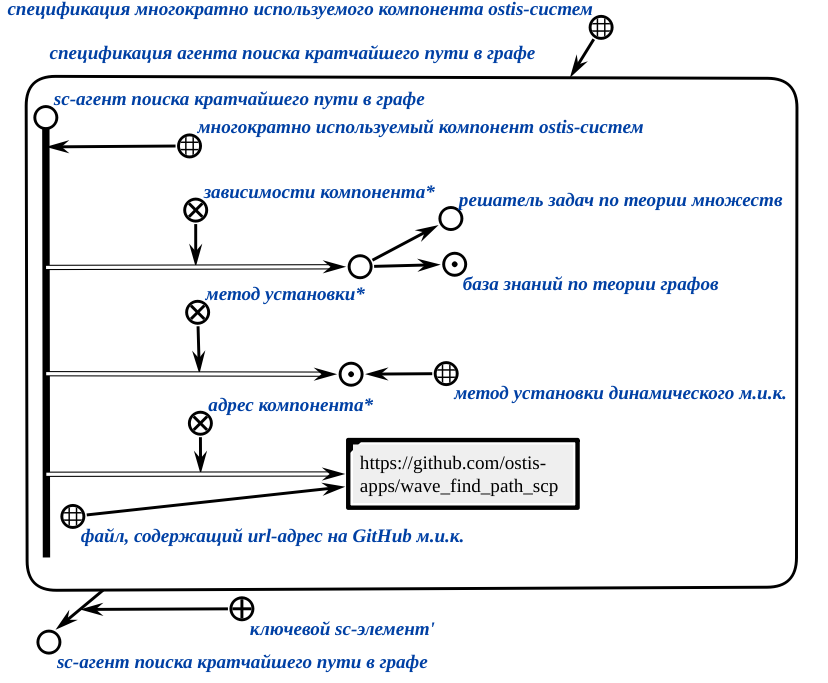
\includegraphics[scale=0.6]{author/part5/figures/component_required_specification_example.png}
	\caption{Пример обязательной части спецификации многократно используемого компонента ostis-систем}
	\label{fig:component_required_specification_example}
\end{figure}

Метод установки позволяет пользователю установить компонент вручную, а \textbf{\textit{менеджеру многократно используемых компонентов ostis-систем}} -- автоматически. Основные два метода установки многократно используемых компонентов -- метод установки \underline{динамически} устанавливаемого многократно используемого компонента ostis-систем и метод установки многократно используемого компонента, при установке которого система \underline{требует перезапуска}. При динамической установке необходимо только скачать компонент и, при необходимости, его зависимые компоненты, и он сразу же функционирует в системе. 

\begin{figure}[H]
	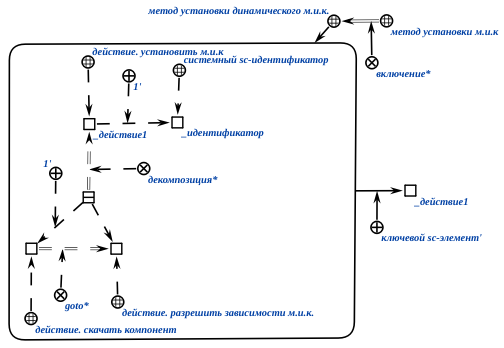
\includegraphics[scale=0.6]{author/part5/figures/install_dynamic_method.png}
	\caption{Метод установки динамически устанавливаемого многократно используемого компонента ostis-систем}
	\label{fig:dynamic_method}
\end{figure}

При установке компонента, при установке которого система требует перезапуска необходимо помимо скачивания компонента транслировать его в память системы.

\begin{figure}[H]
	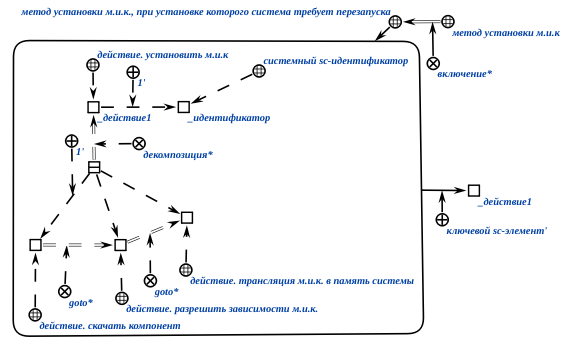
\includegraphics[scale=0.6]{author/part5/figures/install_with_reboot_method.png}
	\caption{Метод установки динамически устанавливаемого многократно используемого компонента, при установке которого система требует перезапуска}
	\label{fig:install_with_reboot_method}
\end{figure}


Связки отношения \textit{адрес хранилища*} связывают многократно используемый компонент, хранящийся в виде внешних файлов и файл, содержащий url-адрес многократно используемого компонента ostis-систем. Таким файлом может быть файл, содержащий url-адрес на GitHub многократно используемого компонента ostis-систем, файл, содержащий url-адрес на Google Drive многократно используемого компонента ostis-систем, файл, содержащий url-адрес на Docker Hub многократно используемого компонента ostis-систем и другие.

Связки отношения \textit{зависимости компонента*} связывают многократно используемый компонент, и множество компонентов, без которых устанавливаемый компонент \underline{не может быть} встроен в дочернюю ostis-систему.

Спецификация неатомарного многократно используемого компонента должна содержать информацию о том, из каких компонентов он состоит, используя отношение \textit{декомпозиция*}. При этом sc-структура, обозначающая неатомарный компонент не обязана содержать все sc-элементы компонентов, на которые она декомпозируется, достаточно, чтобы неатомарному компоненту принадлежали знаки всех тех компонентов, из которых он состоит (должно быть полное перечисление составных компонентов).

На рисунке \nameref{fig:component_optional_specification_example} изображена необязательная часть спецификации, необходимой для установки sc-агента поиска кратчайшего пути в графе. Полная спецификация компонента является результатом объединения обязательной и необязательной частей.

\begin{figure}[H]
	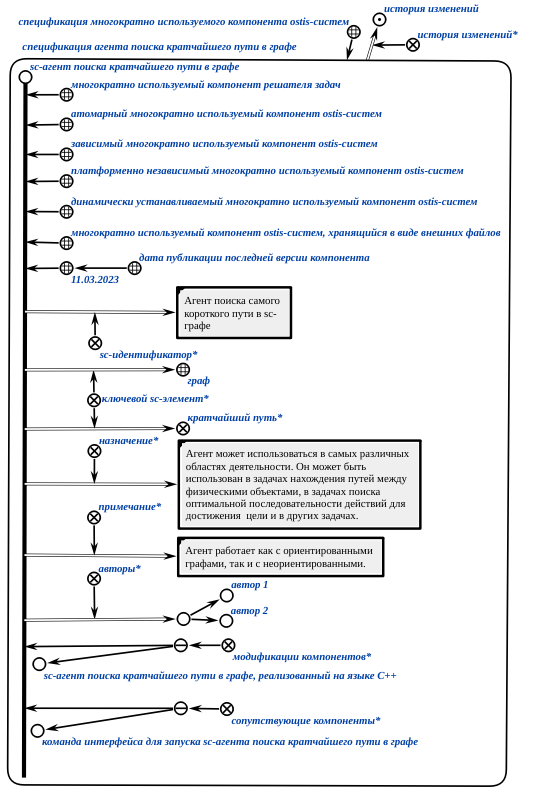
\includegraphics[scale=1.0]{author/part5/figures/component_optional_specification_example.png}
	\caption{Пример необязательной части спецификации многократно используемого компонента ostis-систем}
	\label{fig:component_optional_specification_example}
\end{figure}

В некоторых случаях может оказаться, что для использования одного многократно используемого компонента OSTIS целесообразно или даже необходимо дополнительно использовать несколько других многократно используемых компонентов OSTIS. Например, может оказаться целесообразным вместе с каким либо sc-агентом информационного поиска использовать соответствующую команду интерфейса, которая представлена отдельным компонентом и позволит пользователю задавать вопрос для указанного sc-агента через интерфейс системы. В таких случаях для связи компонентов используется отношение \textit{сопутствующие компоненты*}. Наличие таких связей позволяет устранить возможные проблемы неполноты знаний и навыков в дочерней системе, из-за которых какие-либо из компонентов могут не выполнять свои функции. Связки отношения \textit{сопутствующий компонент*} связывают многократно используемые компоненты ostis-систем, которые целесообразно использовать в дочерней системе вместе. Каждая такая связка может дополнительно быть снабжена sc-комментарием или sc-пояснением, отражающим суть указываемой зависимости. Отношение \textit{история изменений*} позволяет специфицировать различные версии компонента и, при необходимости, устанавливать выбранную пользователем версию. Различные версии, как правило, отражают какие-либо улучшения или исправления ошибок. \textit{Модификации компонентов*} -- это функционально эквивалентные реализации одного и того же компонента, которые могут быть синтаксически эквивалентны (например, реализация одного и того же sc-агента на платформенно-зависимом и пталформенно-независимом уровнях). Развитие Библиотеки OSTIS происходит не только за счёт её пополнения новыми компонентами, но и за счёт появления новых версий и модификаций уже существующих компонентов. Связки отношения \textit{авторы*} связывают многократно используемый компонент со множеством авторов этого компонента. Спецификация может также содержать дополнительную информацию об авторах при необходимости. Отношения \textit{примечание*} и \textit{пояснение*} связывают многократно используемый компонент и некоторый текст (как естественно-языковой, так и текст на языке SC), который является примечанием или пояснением к этому компоненту. Идентификаторы компонента позволяют пользователям и разработчикам обозначать компонент, используя внешний язык. Ключевые sc-элементы компонента позволяют указать на наиболее важные понятия, связанные с описываемым компонентом. Отношение \textit{назначение*} позволяет описать ожидаемый сценарий, выделить рекомендации использования многократно используемого компонента. Требования полноты и безошибочности специфицируют возможные ограничения и ошибки компонента, область его использования.

\section{Менеджер многократно используемых компонентов ostis-систем}
\label{ostis_library_component_manager}

\begin{SCn}
\begin{scnrelfromlist}{ключевое понятие}
	\scnitem{менеджер многократно используемых компонентов ostis-систем}
\end{scnrelfromlist}
\end{SCn}

\bigskip

\begin{SCn}
\begin{scnrelfromlist}{ключевое знание}
	\scnitem{Функциональные возможности менеджера многократно используемых компонентов ostis-систем}
\end{scnrelfromlist}
\end{SCn}

\bigskip

менеджер многократно используемых компонентов ostis-систем -- подсистема ostis-системы, с помощью которой проиходит взаимодействие с библиотекой компонентов ostis-систем.

\begin{SCn}
\scnheader{менеджер многократно используемых компонентов ostis-систем}
\scnidtftext{часто используемый sc-идентификатор}{менеджер многократно используемых компонентов}
\scnidtftext{часто используемый sc-идентификатор}{менеджер компонентов}
\begin{scnrelfromset}{обобщенная декомпозиция}
	\scnitem{база знаний менеджера многократно используемых компонентов ostis-систем}
	\scnitem{решатель задач менеджера многократно используемых компонентов ostis-систем}
	\scnitem{интерфейс менеджера многократно используемых компонентов ostis-систем}
\end{scnrelfromset}
\end{SCn}

База знаний менеджера компонентов содержит все те знания, которые необходимы для установки многократно используемого компонента в дочернюю ostis-систему. К таким знаниям относятся знания о спецификации многократно используемых компонентов, методы установки компонентов, знание о  библиотеках ostis-систем, с которыми происходит взаимодействие. Решатель задач менеджера компонентов взаимодействует с библиотекой ostis-систем и позволяет установить и интегрировать многократно используемые компоненты в дочернюю ostis-систему, также выполнять поиск, обновление, публикацию, удаление компонентов. Интерфейс менеджера многократно используемых компонентов обеспечивает удобное для пользователя и других систем использование менеджера компонентов.

Функциональные возможности менеджера компонентов ostis-систем следующие:
\begin{textitemize}
	\item \textbf{Поиск многократно используемых компонентов ostis-систем}. Множество возможных критериев поиска соответствует спецификации многократно используемых компонентов. Такими критериями могут быть классы компонента, его авторы, идентификатор, фрагмент примечания, назначение, принадлежность какой-либо предметной области, вид знаний компонента и другие.
	\item \textbf{Установка многократно используемого компонента ostis-систем}. Установка многократно используемого компонента происходит вне зависимости от типологии, способа установки и местоположения компонента. Необходимое условие для возможности установки многократно используемого компонента -- наличие \textbf{\textit{спецификации многократно используемого компонента ostis-систем}}. Перед установкой многократно используемого компонента в дочернюю систему необходимо разрешить все зависимости путём установки зависимых компонентов. После успешной установки компонента, в базе знаний дочерней системы генерируется информационная конструкция, обозначающая факт установки компонента в систему с помощью отношения \textit{установленные компоненты*}. После установки компонента в ostis-систему могут возникнуть противоречия в базе знаний, которые  устраняются с помощью средств обнаружения и анализа ошибок и противоречий в базе знаний ostis-системы.
	\item \textbf{Спецификация многократно используемого компонента ostis-систем}. Менеджер компонентов позволяет специфицировать компоненты, входящие в состав библиотеки ostis-систем, а также специфицировать новые создаваемые компоненты, которые будут публиковаться в библиотеку ostis-систем. При этом спецификация может происходить как автоматически, так вручную. Например, менеджер компонентов может обновить спецификацию используемого компонента в соответствии с тем, в какие новые ostis-системы его установили, обновление спецификации авторства компонента при его редактировании в библиотеке ostis-систем, спецификация ошибок, выявленных в процессе эксплуатации компонента и так далее.
	\item \textbf{Формирование многократно используемого компонента ostis-систем по шаблону с заданными параметрами}.
	\item \textbf{Публикация многократно используемого компонента ostis-систем в библиотеку ostis-систем}. При публикации компонента в библиотеку ostis-систем происходит верификация на основе спецификации компонента. Также существует возможность обновления версии опубликованного компонента сообществом его разработчиков.
	\item \textbf{Обновление установленного многократно используемого компонента ostis-систем}
	\item \textbf{Удаление установленного многократно используемого компонента}. Как и в случае установки после удаления многократно используемого компонента из ostis-системы в базе знаний системы устанавливается факт удаления компонента. Эта информация является важной частью \underline{истории эксплуатации} ostis-системы.
	\item \textbf{Редактирование многократно используемого компонента в библиотеке ostis-систем}.
	\item \textbf{Добавление и удаление отслеживаемых ostis-системой библиотек}. Менеджер компонентов содержит информацию о множестве источников для установки компонентов, перечень которых можно дополнять вручную. По умолчанию менеджер компонентов отслеживает Библиотеку Метасистемы OSTIS, однако можно создавать и добавлять дополнительные библиотеки ostis-систем.
	\item \textbf{Сравнение} многократно используемых компонентов ostis-систем.
\end{textitemize}

% Включение компонента в дочернюю sc-систему в самом общем случае состоит из следующих этапов:
% - поиск подходящего компонента (или набора компонентов) во множестве библиотек, входящих в состав IMS. Для облегчения задачи поиска могут быть реализованы специализированные поисковые агенты. В любом случае, поиск и выделение компонента будет осуществляться на основе спецификации компонента. Данный этап с точки зрения пользователя не зависит от типа компонента и особенностей его реализации. Конкретные действия на следующих этапах сильно зависят от реализации и типа компонента и будут более детально описаны при рассмотрении подклассов многократно используемых компонентов OSTIS;

% - выделение компонента (или набора компонентов) в рамках IMS в виде, удобном для транспортировки в дочернюю sc-систему (при необходимости – создание физической копии компонента);

%- транспортировка выделенного компонента в дочернюю sc-систему;

% - интеграция компонента в дочернюю scсистему. Если в системе уже использовалась более старая версия компонента, то необходимо произвести либо локальное обновление, либо полную замену устаревшей версии компонента. Дальнейший процесс интеграции зависит от типа компонента, например, в случае добавления нового sc-агента он должен быть помечен как активный sc-агент и т.п.

% Сказать как устанавливается шаблон компонента -- установление значений переменным происходит в отдельной подсистеме

% Агент сборки многократно используемого компонента.

% Установка компонентов "многократно используемый компонент, хранящийся в виде sc-структуры" и в виде внешних файлов.

%Для обеспечения возможности встраивания многократно используемых компонентов OSTIS в дочернюю систему, каждая такая система обязана иметь в своем составе средства, обеспечивающие интеграцию новых компонентов в систему и, при необходимости, удаление устаревших версий этих компонентов (или автоматического локального обновления компонентов до более новой версии).

\section*{Заключение Главы \ref{chapter_library}}
\label{ostis_library_conclusion}

Компонентный подход к проектированию интеллектуальных компьютерных систем является ключевым в технологии проектирования интеллектуальных компьютерных систем. Вместе с этим, технология компонентного проектирования тесно связана с остальными составляющими технологии проектирования интеллектуальных компьютерных систем и обеспечивает их совместимость, производя мощнейший синергетический эффект при использовании всего комплекса частных технологий проектирования интеллектуальных систем. Важнейшим принципом в реализации компонентного подхода является семантическая совместимость многократно используемых компонентов, что позволяет минимизировать участие программистов в создании новых компьютерных систем и в совершенствовании существующих.

Для реализации компонентного подхода в работе предложена библиотека многократно используемых совместимых компонентов интеллектуальных компьютерных систем на основе Технологии OSTIS, введена классификация и спецификация многократно используемых компонентов ostis-систем, предложена модель менеджера компонентов, позволяющего взаимодействовать ostis-системам с библиотеками многократно используемых компонентов и управлять компонентами в системе, рассмотрена архитектура экосистемы интеллектуальных компьютерных систем с точки зрения использования библиотеки многократно используемых компонентов.

Полученные результаты позволят повысить эффективность проектирования интеллектуальных систем и средств автоматизации разработки таких систем, а также обеспечить возможность не только разработчику, но и интеллектуальной системе автоматически дополнять систему новыми знаниями и навыками.

%%%%%%%%%%%%%%%%%%%%%%%%% referenc.tex %%%%%%%%%%%%%%%%%%%%%%%%%%%%%%
% sample references
% %
% Use this file as a template for your own input.
%
%%%%%%%%%%%%%%%%%%%%%%%% Springer-Verlag %%%%%%%%%%%%%%%%%%%%%%%%%%
%
% BibTeX users please use
% \bibliographystyle{}
% \bibliography{}
%
\biblstarthook{In view of the parallel print and (chapter-wise) online publication of your book at \url{www.springerlink.com} it has been decided that -- as a genreral rule --  references should be sorted chapter-wise and placed at the end of the individual chapters. However, upon agreement with your contact at Springer you may list your references in a single seperate chapter at the end of your book. Deactivate the class option \texttt{sectrefs} and the \texttt{thebibliography} environment will be put out as a chapter of its own.\\\indent
References may be \textit{cited} in the text either by number (preferred) or by author/year.\footnote{Make sure that all references from the list are cited in the text. Those not cited should be moved to a separate \textit{Further Reading} section or chapter.} If the citatiion in the text is numbered, the reference list should be arranged in ascending order. If the citation in the text is author/year, the reference list should be \textit{sorted} alphabetically and if there are several works by the same author, the following order should be used:
\begin{enumerate}
\item all works by the author alone, ordered chronologically by year of publication
\item all works by the author with a coauthor, ordered alphabetically by coauthor
\item all works by the author with several coauthors, ordered chronologically by year of publication.
\end{enumerate}
The \textit{styling} of references\footnote{Always use the standard abbreviation of a journal's name according to the ISSN \textit{List of Title Word Abbreviations}, see \url{http://www.issn.org/en/node/344}} depends on the subject of your book:
\begin{itemize}
\item The \textit{two} recommended styles for references in books on \textit{mathematical, physical, statistical and computer sciences} are depicted in ~\cite{science-contrib, science-online, science-mono, science-journal, science-DOI} and ~\cite{phys-online, phys-mono, phys-journal, phys-DOI, phys-contrib}.
\item Examples of the most commonly used reference style in books on \textit{Psychology, Social Sciences} are~\cite{psysoc-mono, psysoc-online,psysoc-journal, psysoc-contrib, psysoc-DOI}.
\item Examples for references in books on \textit{Humanities, Linguistics, Philosophy} are~\cite{humlinphil-journal, humlinphil-contrib, humlinphil-mono, humlinphil-online, humlinphil-DOI}.
\item Examples of the basic Springer style used in publications on a wide range of subjects such as \textit{Computer Science, Economics, Engineering, Geosciences, Life Sciences, Medicine, Biomedicine} are ~\cite{basic-contrib, basic-online, basic-journal, basic-DOI, basic-mono}. 
\end{itemize}
}

\begin{thebibliography}{99.}%
% and use \bibitem to create references.
%
% Use the following syntax and markup for your references if 
% the subject of your book is from the field 
% "Mathematics, Physics, Statistics, Computer Science"
%
% Contribution 
\bibitem{science-contrib} Broy, M.: Software engineering --- from auxiliary to key technologies. In: Broy, M., Dener, E. (eds.) Software Pioneers, pp. 10-13. Springer, Heidelberg (2002)
%
% Online Document
\bibitem{science-online} Dod, J.: Effective substances. In: The Dictionary of Substances and Their Effects. Royal Society of Chemistry (1999) Available via DIALOG. \\
\url{http://www.rsc.org/dose/title of subordinate document. Cited 15 Jan 1999}
%
% Monograph
\bibitem{science-mono} Geddes, K.O., Czapor, S.R., Labahn, G.: Algorithms for Computer Algebra. Kluwer, Boston (1992) 
%
% Journal article
\bibitem{science-journal} Hamburger, C.: Quasimonotonicity, regularity and duality for nonlinear systems of partial differential equations. Ann. Mat. Pura. Appl. \textbf{169}, 321--354 (1995)
%
% Journal article by DOI
\bibitem{science-DOI} Slifka, M.K., Whitton, J.L.: Clinical implications of dysregulated cytokine production. J. Mol. Med. (2000) doi: 10.1007/s001090000086 
%
\bigskip

% Use the following (APS) syntax and markup for your references if 
% the subject of your book is from the field 
% "Mathematics, Physics, Statistics, Computer Science"
%
% Online Document
\bibitem{phys-online} J. Dod, in \textit{The Dictionary of Substances and Their Effects}, Royal Society of Chemistry. (Available via DIALOG, 1999), 
\url{http://www.rsc.org/dose/title of subordinate document. Cited 15 Jan 1999}
%
% Monograph
\bibitem{phys-mono} H. Ibach, H. L\"uth, \textit{Solid-State Physics}, 2nd edn. (Springer, New York, 1996), pp. 45-56 
%
% Journal article
\bibitem{phys-journal} S. Preuss, A. Demchuk Jr., M. Stuke, Appl. Phys. A \textbf{61}
%
% Journal article by DOI
\bibitem{phys-DOI} M.K. Slifka, J.L. Whitton, J. Mol. Med., doi: 10.1007/s001090000086
%
% Contribution 
\bibitem{phys-contrib} S.E. Smith, in \textit{Neuromuscular Junction}, ed. by E. Zaimis. Handbook of Experimental Pharmacology, vol 42 (Springer, Heidelberg, 1976), p. 593
%
\bigskip
%
% Use the following syntax and markup for your references if 
% the subject of your book is from the field 
% "Psychology, Social Sciences"
%
%
% Monograph
\bibitem{psysoc-mono} Calfee, R.~C., \& Valencia, R.~R. (1991). \textit{APA guide to preparing manuscripts for journal publication.} Washington, DC: American Psychological Association.
%
% Online Document
\bibitem{psysoc-online} Dod, J. (1999). Effective substances. In: The dictionary of substances and their effects. Royal Society of Chemistry. Available via DIALOG. \\
\url{http://www.rsc.org/dose/Effective substances.} Cited 15 Jan 1999.
%
% Journal article
\bibitem{psysoc-journal} Harris, M., Karper, E., Stacks, G., Hoffman, D., DeNiro, R., Cruz, P., et al. (2001). Writing labs and the Hollywood connection. \textit{J Film} Writing, 44(3), 213--245.
%
% Contribution 
\bibitem{psysoc-contrib} O'Neil, J.~M., \& Egan, J. (1992). Men's and women's gender role journeys: Metaphor for healing, transition, and transformation. In B.~R. Wainrig (Ed.), \textit{Gender issues across the life cycle} (pp. 107--123). New York: Springer.
%
% Journal article by DOI
\bibitem{psysoc-DOI}Kreger, M., Brindis, C.D., Manuel, D.M., Sassoubre, L. (2007). Lessons learned in systems change initiatives: benchmarks and indicators. \textit{American Journal of Community Psychology}, doi: 10.1007/s10464-007-9108-14.
%
%
% Use the following syntax and markup for your references if 
% the subject of your book is from the field 
% "Humanities, Linguistics, Philosophy"
%
\bigskip
%
% Journal article
\bibitem{humlinphil-journal} Alber John, Daniel C. O'Connell, and Sabine Kowal. 2002. Personal perspective in TV interviews. \textit{Pragmatics} 12:257--271
%
% Contribution 
\bibitem{humlinphil-contrib} Cameron, Deborah. 1997. Theoretical debates in feminist linguistics: Questions of sex and gender. In \textit{Gender and discourse}, ed. Ruth Wodak, 99--119. London: Sage Publications.
%
% Monograph
\bibitem{humlinphil-mono} Cameron, Deborah. 1985. \textit{Feminism and linguistic theory.} New York: St. Martin's Press.
%
% Online Document
\bibitem{humlinphil-online} Dod, Jake. 1999. Effective substances. In: The dictionary of substances and their effects. Royal Society of Chemistry. Available via DIALOG. \\
http://www.rsc.org/dose/title of subordinate document. Cited 15 Jan 1999
%
% Journal article by DOI
\bibitem{humlinphil-DOI} Suleiman, Camelia, Daniel C. O'Connell, and Sabine Kowal. 2002. `If you and I, if we, in this later day, lose that sacred fire...': Perspective in political interviews. \textit{Journal of Psycholinguistic Research}. doi: 10.1023/A:1015592129296.
%
%
%
\bigskip
%
%
% Use the following syntax and markup for your references if 
% the subject of your book is from the field 
% "Computer Science, Economics, Engineering, Geosciences, Life Sciences"
%
%
% Contribution 
\bibitem{basic-contrib} Brown B, Aaron M (2001) The politics of nature. In: Smith J (ed) The rise of modern genomics, 3rd edn. Wiley, New York 
%
% Online Document
\bibitem{basic-online} Dod J (1999) Effective Substances. In: The dictionary of substances and their effects. Royal Society of Chemistry. Available via DIALOG. \\
\url{http://www.rsc.org/dose/title of subordinate document. Cited 15 Jan 1999}
%
% Journal article by DOI
\bibitem{basic-DOI} Slifka MK, Whitton JL (2000) Clinical implications of dysregulated cytokine production. J Mol Med, doi: 10.1007/s001090000086
%
% Journal article
\bibitem{basic-journal} Smith J, Jones M Jr, Houghton L et al (1999) Future of health insurance. N Engl J Med 965:325--329
%
% Monograph
\bibitem{basic-mono} South J, Blass B (2001) The future of modern genomics. Blackwell, London 
%
\end{thebibliography}

\chapter{Методика и средства проектирования и анализа качества баз знаний ostis-систем}
\chapauthortoc{Бутрин С.В.\\Шункевич Д.В.\\Банцевич К.А.}
\label{chapter_kb_design}

\vspace{-7\baselineskip}

\scntext{эпиграф}{Дырявая и запутанная сеть хорошего улова не принесет.}

\begin{SCn}
	\begin{scnrelfromlist}{автор}
		\scnitem{Бутрин С.В.}
		\scnitem{Шункевич Д.В.}
		\scnitem{Банцевич К.А.}
	\end{scnrelfromlist}

\bigskip

\scntext{аннотация}{В главе рассматриваются актуальные проблемы текущего состояния средств проектирования и анализа качества \textit{баз знаний}, предложен подход к их решению на основе \textit{Технологии OSTIS}. Сформулированы принципы коллективного проектирования и разработки \textit{баз знаний}. Сформулированы принципы верификации \textit{баз знаний}.}

\bigskip

\begin{scnrelfromlist}{подраздел}
	\scnitem{\ref{sec_kb_design_methods}~\nameref{sec_kb_design_methods}}
	\scnitem{\ref{sec_kb_design_individual}~\nameref{sec_kb_design_individual}}	\scnitem{\ref{sec_kb_design_collective}~\nameref{sec_kb_design_collective}}
	\scnitem{\ref{sec_kb_design_contradiction}~\nameref{sec_kb_design_contradiction}}
	\scnitem{\ref{sec_kb_design_developers}~\nameref{sec_kb_design_developers}}
	\scnitem{\ref{sc_kb_design_components}~\nameref{sc_kb_design_components}}
\end{scnrelfromlist}

\bigskip

\begin{scnrelfromlist}{ключевое понятие}
	\scnitem{база знаний}
	\scnitem{редактор баз знаний}
	\scnitem{разработка баз знаний}
	\scnitem{разработчик}
	\scnitem{противоречие}
	\scnitem{информационная дыра}
	\scnitem{многократно используемые компоненты}
\end{scnrelfromlist}

\bigskip

\begin{scnrelfromlist}{библиографическая ссылка}
	\scnitem{\scncite{Arshinskiy2020}}
	\scnitem{\scncite{Rybina2007}}
	\scnitem{\scncite{Zhang2023}}
	\scnitem{\scncite{Davydenko2016}}
	\scnitem{\scncite{Davydenko2017}}
	\scnitem{\scncite{Davydenko2018}}
\end{scnrelfromlist}

\end{SCn}

\section*{Введение в Главу \ref{chapter_kb_design}}

Разработка базы знаний является трудоемким и продолжительным процессом, требующим высокого уровня квалификации разработчиков баз знаний. Данный факт приводит к высокой себестоимости как самих баз знаний, так и соответствующих им интеллектуальных систем, а также к дефициту специалистов в области инженерии знаний.

Расширение областей применения интеллектуальных систем требует поддержки решения комплексных задач.
Решение каждой такой задачи предполагает совместное использование различных видов знаний и моделей их представления, что приводит к компенсации недостатков одних моделей возможностями и достоинствами других.

Cуществующие средства создания баз знаний предполагают, что процессы разработки и модификации базы знаний осуществляются отдельно от процесса ее использования, что приводит к дополнительному усложнению решения задачи обеспечения совместимости различного вида знаний.
Отсутствие удовлетворительного решения этой задачи приводит к несовместимости компонентов баз знаний, разрабатываемых для разных систем, и невозможности их повторного использования в других системах.
Данный факт приводит к многократной повторной разработке содержательно одних и тех же компонентов для разных баз знаний.

Таким образом, актуальной является задача разработки модели баз знаний, которая, с одной стороны, обеспечит общий унифицированный формальный фундамент для представления различных видов знаний в рамках одной базы знаний и их совместного использования при решении комплексных задач, а с другой стороны, обеспечит возможность расширения числа видов знаний, используемых интеллектуальной системой (См. \scncite{Davydenko2016}). 


\section{Действия и методики проектирования баз знаний ostis-систем}
\label{sec_kb_design_methods}

\textit{База знаний} является ключевым компонентом интеллектуальной системы, которая в систематизированном виде включает в себя все знания, необходимые интеллектуальной системе для ее функционирования.

Для задач, решаемых интеллектуальными системами, в общем случае неизвестно, какие данные и знания должны быть использованы для решения этих задач, какие должны быть использованы способы их решения.
При решении таких задач необходима локализация фрагмента базы знаний, содержащего данные и знания, достаточные для решения задачи, и исключающего те данные и знания, которые заведомо для этого не нужны, а также выделение из имеющегося многообразия способов решения задач тех способов, которых достаточно для решения данной задачи.

Однако для обеспечения совместного использования различных видов знаний в единой базе знаний необходимо обеспечить совместимость этих видов знаний и, как следствие, совместимость компонентов баз знаний, которая включает два аспекта: обеспечение синтаксической совместимости, что подразумевает унификацию формы представления знаний, и обеспечение семантической совместимости, что подразумевает однозначную и единую для всех компонентов трактовку используемых понятий.

Существующие подходы к разработке баз знаний, как правило, предполагают решение задачи обеспечения синтаксической совместимости знаний путем соединения разнородных моделей представления знаний, а также разработки новых интегрированных моделей и новых языков представления знаний.
Разработка базы знаний таким способом приводит к дополнительным накладным расходам при интеграции и обработке разнородных знаний, и, как следствие, к резкому увеличению трудозатрат при модификации таких баз знаний и добавлении новых видов знаний.
Таким образом, интеллектуальная система, способная решать комплексные задачи, должна обладать способностью приобретать новые знания и навыки в процессе ее эксплуатации, сохраняя при этом корректность и целостность базы знаний.

В свою очередь, это обуславливает требование модицифируемости к такой базе знаний, то есть снижения трудоемкости внесения изменений в базу знаний.
Таким образом, можно сформулировать требования к базе знаний систем, способных решать комплексные задачи:

\begin{textitemize}
\item возможность согласованного использования различных видов знаний, хранимых в одной базе знаний, при решении каждой комплексной задачи;

\item возможность реализации различных аспектов спецификации сущностей, описываемых в базе знаний;

\item модифицируемость базы знаний, позволяющая непосредственно в процессе эксплуатации интеллектуальной системы добавлять в базу знаний новые фрагменты, в том числе новые виды знаний без внесения изменений в существующую структуру базы знаний;

\item возможность неограниченного перехода в рамках каждой базы знаний от знаний к метазнаниям, от метазнаний к метаметазнаниям и т. д., что, в частности, предоставляет неограниченные возможности типологии и систематизации знаний, хранимых в составе базы знаний, и неограниченные возможности декомпозиции и структуризации самой базы знаний;

\item наличие языковых средств, позволяющих в рамках базы знаний представлять метазнания, описывающие качество базы знаний (противоречия, неполноту, избыточность);

\item наличие языковых средств, позволяющих в рамках базы знаний представлять метазнания, описывающие историю эволюции и планы дальнейшей эволюции базы знаний;

\item возможность для каждой решаемой задачи явно задавать и уточнять в ходе решения задачи область решения, то есть такой фрагмент базы знаний, использование которого является достаточным для решения этой задачи.
\end{textitemize}

А также следующие дополнительные требования к функциональности системы поддержки коллективной разработки гибридных баз знаний, учитывающие недостатки рассмотренных аналогов:

\begin{textitemize}
\item обеспечение возможности как ручного, так и автоматического редактирования баз знаний;

\item обеспечение возможности автоматической верификации базы знаний, в том числе анализ корректности и полноты базы знаний;

\item обеспечение возможности создания базы знаний распределенным коллективом разработчиков, включая механизм согласования вносимых в базу знаний изменений, а также механизм хранения истории вносимых изменений с указанием авторства.
\end{textitemize}

Реализация перечисленных возможностей подразумевает отказ от работы с файлами исходными текстами базы знаний. В данном случае предполагается, что все изменения осуществляются непосредственно в памяти системы, где хранится вся база знаний, что позволяет осуществлять разработку базы знаний компьютерной системы в процессе ее эксплуатации (См. \scncite{Davydenko2017}).

%%%%%%%%%%%%%%%%%%%%

Проектирование базы знаний включает в себя два аспекта: индивидуальный и коллективный.
Индивидульный представляет собой наполнение изолировнной части базы знаний конкретным пользователем.
Коллективный представляет собой согласование все базы знаний и включает в себя процесс внедрения изменений и внесения предложений.

Таким образом индивидуальный аспект включает в себя средства и методы позволяющие пользователю непосредственно наполнять базу знаний посредствам редакторов, трансляторов и т.д. При этом процесс редактирования базы знаний должен быть максимально удобным и понятным для пользователя.

Коллективный же аспект включает в себя средства и методы для автоматического или полуавтоматического согласования общей базы знаний с индивидуальными базами знаний пользователей. То есть он включает в себя процессы создания предложений по изменению базы знаний, их рассмотрение и внесение в общую базу знаний.

Так как в основе любой современной базы знаний лежат онтологии, то методы и средства разработки онтологий являются важнейшей частью технологий разработки баз знаний.
Методология разработки онтологий представляет собой набор инструкций и руководств, описывающих процесс выполнения сложных процедур разработки онтологий.
Она детализирует различные задачи, как они должны бытьвыполнены, в каком порядке и каким образом осуществлять документирование работы по созданию онтологий.
Существующие методологии можно условно разделить на представленные ниже группы.

\begin{SCn}
\scnheader{методология разработки онтологий}
\scnrelfrom{разбиение}{\scnkeyword{Типология методологий по поддержке коллективной разработки\scnsupergroupsign}}
\begin{scnindent}
	\begin{scneqtoset}
		\scnitem{методология, поддерживающая совместную коллективную разработку онтологии}
		\scnitem{методология, поддерживающая совместную коллективную разработку онтологии}
		\scnitem{методология, не поддерживающая совместную коллективную разработку онтологии}
	\end{scneqtoset}
\end{scnindent}

\scnrelfrom{разбиение}{\scnkeyword{Типология методологий по степени зависимости от инструментария\scnsupergroupsign}}
\begin{scnindent}
	\begin{scneqtoset}
		\scnitem{методология, зависимая от инструментария}
		\scnitem{методология, полузависимая от инструментария}
		\scnitem{методология, независимая от инструментария}
	\end{scneqtoset}
\end{scnindent}

\scnrelfrom{разбиение}{\scnkeyword{Типология методологий по типу используемой модели жизненного цикла онтологии\scnsupergroupsign}}
\begin{scnindent}
	\begin{scneqtoset}
		\scnitem{методология без указания модели жизненного цикла онтологии}
		\scnitem{методология с итеративной моделью жизненного цикла онтологии}
		\scnitem{методология с моделью жизненного цикла онтологии на основе эволюционного прототипирования}
		\scnitem{методология с совпадающей с моделью жизненного цикла приложения}
	\end{scneqtoset}
\end{scnindent}

\scnrelfrom{разбиение}{\scnkeyword{Типология методологий по возможности формализации\scnsupergroupsign}}
\begin{scnindent}
	\begin{scneqtoset}
		\scnitem{методология, предусматривающие способы формализации}
		\scnitem{методология, не предусматривающие формализации}
	\end{scneqtoset}
\end{scnindent}

\scnrelfrom{разбиение}{\scnkeyword{Типология методологий по возможности повторного использования разрабатываемых онтологий\scnsupergroupsign}}
\begin{scnindent}
	\begin{scneqtoset}
		\scnitem{методология, поддерживающие повторное использование}
		\scnitem{методология, не поддерживающие повторного использования}
	\end{scneqtoset}
\end{scnindent}

\scnrelfrom{разбиение}{\scnkeyword{Типология методологий по стратегии выделения концептов предметной области\scnsupergroupsign}}
\begin{scnindent}
	\begin{scneqtoset}
		\scnitem{методология снизу вверх (bottom-up)}
		\scnitem{методология сверху вниз (top-down)}
		\scnitem{методология от середины (middle-out)}
		\scnitem{методология сочетающие различные стратегии}
	\end{scneqtoset}
\end{scnindent}

\scnrelfrom{разбиение}{\scnkeyword{Типология методологий по возможности поддержки совместимости разрабатываемых онтологий\scnsupergroupsign}}
\begin{scnindent}
	\begin{scneqtoset}
		\scnitem{методология, поддерживающая совместимость}
		\scnitem{методология, не поддерживающая совместимость}
	\end{scneqtoset}
\end{scnindent}

\end{SCn}

Большинство методологий не поддерживают совместную разработку баз знаний, поддержку совместимости разрабатываемых баз знаний и, как следствие, поддержку повторного использования уже разработанных баз знаний и их компонентов.

Кроме того, подавляющее большинство методологий разработки баз знаний описывают процесс разработки в общих чертах, не регламентируя действия участников на каждом этапе разработки онтологии, не уточняя принципы согласования новых понятий с уже существующими, высоким оказывается субъективное влияние разработчиков.

%%%%%%%%%%%%%%%%%%%%%%%

Отличительной особенностью предлагаемой методики от существующих методологий разработки баз знаний является совершенствование базы знаний коллективом разработчиков непосредственно в процессе ее использования, а также создание новых и использование уже имеющихся компонентов баз знаний в процессе разработки каждой базы знаний.

Данная методика предполагает два основных этапа – этап создания стартовой версии разрабатываемой ostis-системы, база знаний которой синтезируется из компонентов, входящих в библиотеку многократно используемых компонентов баз знаний ostis-систем, и этап расширения и совершенствования базы знаний разрабатываемой ostis-системы, осуществляемый в рамках этой системы.

Стартовая версия ostis-системы содержит набор знаний и средств решения задач, достаточный для дальнейшего развития системы.

Процесс создания стартовой версии ostis-системы можно разделить четыре основных этапа:
\begin{textitemize}
\item выбор и установка \textit{ostis-платформы} для интерпретации sc-модели ostis-системы;

\item установка Ядра sc-модели базы знаний ostis-системы из Библиотеки многократно используемых компонентов баз знаний;

\item установка Ядра решателей задач из Библиотеки многократно используемых компонентов решателей задач, то есть набора базовых многократно используемых компонентов решателей задач, необходимых для работы стартовой версии ostis-системы;

\item установка Ядра sc-моделей интерфейсов, то есть набора базовых многократно используемых компонентов sc-моделей интерфейсов, необходимых для работы стартовой версии ostis-системы;

\item установка системы поддержки коллективной разработки гибридных баз знаний.
\end{textitemize}

Процесс разработки базы знаний включает в себя следующие стадии:
\begin{textitemize}
	\item Формирование начальной структуры гибридной базы знаний, которая предполагает:
		\begin{textitemize}
			\item  формирование структуры разделов базы знаний, соответствующей варианту структуризации базы знаний с точки зрения разработчиков, описан-ному в подразделе 2.6.3 данной диссертационной работы;
			\item выявление описываемых предметных областей;
			\item построение иерархической системы описываемых предметных областей;
			\item построение иерархии разделов базы знаний в рамках предметной	части базы знаний, учитывающей построенную на предыдущем этапе иерархию предметных областей.
		\end{textitemize}
	\item Выявление компонентов базы знаний, которые могут быть заимствованы из библиотеки многократно используемых компонентов баз знаний, и включение их в состав разрабатываемой базы знаний;
	\item Формирование проектных заданий на разработку недостающих фрагментов базы знаний и распределение заданий между разработчиками;
	\item Разработка и согласование фрагментов базы знаний, которые, в свою	очередь, могут в дальнейшем быть включены в состав библиотеки многократно используемых компонентов баз знаний;
	\item Верификация и отладка базы знаний.
\end{textitemize}

Следует отметить, что в процессе совершенствования базы знаний этапы 3 - 5 выполняются циклически.

Для обеспечения свойства рефлексивности интеллектуальной системы, в частности, возможности автоматизации анализа истории эволюции базы знаний и генерации планов по ее развитию, вся деятельность, связанная с разработкой базы знаний, должна специфицироваться в самой этой базе знаний теми же средствами, что и предметная часть (см. \scncite{Davydenko2018}).

\section{Индивидуальный аспект проектирования и разработки баз знаний ostis-систем}
\label{sec_kb_design_individual}

Для решения задачи индивудуального наполения базы знаний прдлагается использовать специализированный инструментарий, который включает в себя различного рода редакторы и трансляторы.

Текущая реализация \textit{ostis-платформы} и решателя задач поддерживает работу с файлами исходных текстов базы знаний.

Для создания таких файлов исходных текстов на SCs-коде можно воспользоваться любым текстовы редактором.

%% Можно добавить иллюстрацию

Для создания файлов исходных текстов на SCg-коде предлагается использовать KBE (Knowledge Base source Editor)(См. \scncite{Knowledge-base-editor2022}). 

Knowledge Base source Editor является приложением, которое направлено на помощь в создании и редактировании фрагментов баз знаний интеллектуальных систем, проектирование которых основано на технологии OSTIS.

В основу данного редактора положен принцип визуализации данных, хранящихся в базе знаний, что намного упрощает процесс их редактирования и ускоряет процесс проектирования баз знаний.

Пользовательский интерфейс инструмента представляет собой главное окно, в котором пользователь может создавать вкладки.

В каждой вкладке может происходить редактирование различных файлов исходных текстов баз знаний представленных с помощью SCg-кода.

В рамках главного окна имеется панель инструментов, и меню приложения. 

Меню приложения представляет собой некоторый набор команд. Команды, которые отображаются в меню делятся на два типа:
\begin{textitemize}
\item команды, которые являются общими для всех вкладок. В частности к ним относятся команды сохранения, загрузки, помощи и т. д.
\item команды, которые специфичны для активной вкладки. Зависят от типа активной вкладки.
\end{textitemize}

На панель инструментов, как и в пользовательских интерфейсах большинства приложений, вынесены наиболее часто используемые команды:
\begin{textitemize}
\item Создать новый файл;
\item Открыть файл;
\item Сохранить;
\item Сохранить как;
\item Закрыть.
\end{textitemize}

Основная идея, которая преследуется в данном редакторе SCg-текстов - это упрощение и ускорение процесса редактирования SCg-текстов.

В процессе редактирования пользователю доступны различные режимы редактирования.

Всего выделено 4 режима:
\begin{textitemize}
\item Режим выделения и создания узлов.
В данном режиме пользователь может работать со всеми объектами выделяя и перемещая их, вызывая контекстное меню с командами.
Отличительной особенностью данного режима является то, что в нем можно создавать sc.g-узлы.

\item Режим создания sc.g-дуг.
Создание sc.g-дуги начинается с того, что пользователь указывает объект из которого она будет выходить, далее он может указать точки излома дуги, завершается создание указанием конечного объекта.
В процессе создания пользователь может отменять последнее действие (указание начального объекта, точки излома);

\item Режим создания sc.g-шин.
sc.g-шины используются для увелечения контактной площади узла, поэтому они могут создаваться лишь для sc.g-узлов. 
Создание шины начинается с указания sc.g-узла, далее как и при создании sc.g-дуг указываются точки излома. 
Как и при создании дуг пользователь может отменять последнее дей-
ствие нажатием правой клавиши мыши;

\item Режим создания sc.g-контуров.
Создание sc.g-контура начинается с указаний первой его точки. Далее, как и в случае с sc.g-дугами и sc.g-шинами, указываются точки.
Стоит отметить, что все объекты, которые попадут внутрь созданного
контура, будут добавлены в него автоматически.
Как и при создании дуг и шин пользователь может отменять последнее действие.
\end{textitemize}

Кроме перечиленных выше команд существует еще целый ряд команд редактирования:
\begin{textitemize}
\item Команда изменения основного текстового идентификатора элемента;
\item Команда изменения типа элемента;
\item Команда установки содержимого.
\end{textitemize}

Полученный файлы исходных текстов в дальнейшем могут быть погружены в базу знаний ostis-системы с помощью \textit{Реализации транслятора файлов исходных текстов базы знаний в sc-память ostis-платформы}.

\begin{SCn}
\scnheader{Реализация транслятора файлов исходных текстов базы знаний в sc-память ostis-платформы}
\scniselement{многократно используемый компонент ostis-систем, хранящийся в виде файлов исходных текстов}

\scnidtf{sc-builder}
\scnrelfrom{используемый язык}{SCs-код}
\begin{scnrelfromset}{зависимости компонента}
	\scnitem{Реализация sc-памяти в ostis-платформе}
	\scnitem{Библиотека методов и структура данных C++ Standart Library}
\end{scnrelfromset}
\scntext{пояснение}{\textit{Реализация транслятора файлов исходных текстов базы знаний в sc-память ostis-платформы} позволяет осуществить сборку базы знаний из набора файлов исходных текстов, записанных в SCs-коде с ограничениями в бинарный формат, воспринимаемый \textit{Программной моделью sc-памяти} (См. \ref{sec_soft_platform_scin_code_example}). При этом возможна как сборка \scnqq{с нуля} (с уничтожением ранее созданного слепка памяти), так и аддитивная сборка, когда информация, содержащаяся в заданном множестве файлов, добавляется к уже имеющемуся слепку состояния памяти.
В текущей реализации сборщик осуществляет \scnqq{склеивание} (\scnqq{слияние}) sc-элементов, имеющих на уровне файлов исходных текстов одинаковые \textit{системные sc-идентификаторы}.}
\end{SCn}

Так же имеется редактор текстов базы знаний, являющийся частью \textit{Реализации интерпретатора sc-моделей пользовательских интерфейсов ostis-систем в Программном варианте реализации ostis-платформы}, обладающий схожим с KBE функционалом, но при этом позволяющий редактировать базу знаний в режиме реального времени и без создания файлов исходных файлов.

\section{Коллективный аспект проектирования и разработки баз знаний ostis-систем}
\label{sec_kb_design_collective}

Для решения задачи коллективной разработки баз знаний разработана модель деятельности, направленной на создание гибридных баз знаний коллективом разработчиков.

Данная модель базируется на модели деятельности различных субъектов и реализована в виде онтологии предметной области деятельности разработчиков, направленной на разработку и модификациюгибридных баз знаний.

Процесс создания и редактирования базы знаний ostis-системы сводится к формированию разработчиками предложений по редактированию того или иного раздела базы знаний и последующему рассмотрению этих предложений администраторами базы знаний.

Кроме того, предполагается, что в случае необходимости для верификации поступающих предложений по редактированию базы знаний могут привлекаться эксперты, а управление процессом разработки осуществляется менеджерами соответствующих проектов по разработке базы знаний.

При этом формирование проектных заданий и их спецификация осуществляются также при помощи механизма предложений по редактированию соответствующего раздела базы знаний. 

Таким образом, вся информация, связанная с текущими процессами разработки базы знаний, историей и планами ее развития, хранится в той же базе знаний, что и ее предметная часть, то есть часть базы знаний, доступная конечному пользователю системы. Такой подход обеспечивает широкие возможности автоматизации процесса создания баз знаний, а также последующего анализа и совершенствования базы знаний.

Каждое предложение по редактированию базы знаний представляет собой структуру, содержащую sc-текст, который предлагается включить в состав согласованной части базы знаний. В состав таких предложений могут входить знаки действий по редактированию базы знаний, которые автоматически инициируются и выполняются соответствующими агентами после утверждения предложения.


\section{Логико-семантическая модель ostis-системы обнаружения и анализа ошибок и противоречий в базе знаний ostis-системы}
\label{sec_kb_design_contradiction}

Важным этапом в разработке любой системы является контроль качества, так как именно на этом этапе определяется степень жизнеспособности и эффективности системы.

Верификация является видом анализа качества и часть процесса разработки. Она заключается в проверке информации на правильность и точность.
Ее целью является выявление ошибок, различных дефектов и недоработок для своевременного их устранения.

Cуществующие на данный момент методы верификации хорошо развиты и разработано большое количество различных моделей верификации, использующих расширенные таблицы решения, сети Петри, различные логики, например, логики с векторной семантикой (см. \scncite{Arshinskiy2020}) и другие модели. Более того формируются специализированные онтологии для описания многообразия средств и моделей верификации баз знаний (см. \scncite{Rybina2007}). Однако механизма взаимодействия средств, использующих данные методы, нет.

Поэтому средства верификации баз знаний, существующие на данный момент, обладают рядом таких проблем как (см. \scncite{Zhang2023}):
\begin{textitemize}
    \item зависимость от формата представления информации, из-за чего приходится тратить дополнительно время на конвертирование информацию
    \item проблема невозможности быть переиспользованными, так как средства обычно делаются с учетом особенностей конкретной системы
    \item проблема отсутствия механизма взаимодействия средств верификации и анализа знаний
    \item высокая роль человека в процессе верификации, так как самым распространенным способом верификации баз знаний является ручная проверка базы экспертом, человек выступает как администратор, принимающий единогласное решение, навязывая свое мнение системе
    \item современные средства не учитывают и не рассматривают процесс верификации в рамках взаимодействия систем друг с другом.
\end{textitemize}

Эти проблемы могли бы быть решены, если:
\begin{textitemize}
    \item использовать унифицированный и удобный формат представления знаний
    \item системы создавались бы по общей методологии и были бы совместимы друг с другом
    \item продумать и реализовать механизм позволяющий системе стремиться самой принимать решение относительно своего состояния и наличия в нем проблемных моментов и ошибок, система может допускать ошибки и не всегда принимать верные решения, но это должны быть ее ошибки, а не экспертов и разработчиков
\end{textitemize}

Преимуществами Технологии OSTIS в рамках задачи верификации являются:
\begin{textitemize}
    \item наличие общей методологии проектирования интеллектуальных систем, позволяющая решить проблему совместимости систем при их коллективном взаимодействии;
    \item все знания представлены в унифицированном виде, что позволяет эффективно их обрабатывать, сводя затраты на конвертирование к минимуму;
   \item средства, с помощью которых производится выявление, анализ и устранение противоречий описаны в самой базе знаний, а так же их спецификация представлены в самой базе знаний системы, тем самым обеспечивая легкость их расширения и позволяя системе знать, каким инструментарием она обладает;
   \item отсутствие семантических эквивалентных фрагментов, что обеспечивает локальность вносимых исправлений и исключает необходимость вносить исправления многократно в разных местах;
   \item многоагентный подход, который позволяет рассматривать средства анализа и верификации баз знаний как коллектив агентов, способных взаимодействовать друг с другом и дальнейшем принимать общее решение касательно состояния базы знаний. 
\end{textitemize}

Предлагаемый подход сводится к разработке:
\begin{textitemize}
    \item специализированной \textit{предметной области и онтологии}, которая бы содержала бы в себе все необходимые знания о возможных видах проблемных фрагментов базы знаний и способах их исправления
    \item алгоритма, позволяющего системе выявить в себе проблемные фрагменты и устранить их, при этом обеспечив согласованность работы средств самой системы
    \item специализированного решателя задач, содержащего необходимые агенты для выявления и устранения проблемных фрагментов
\end{textitemize}

%% ССылки и объяснение что есть что
Качество базы знаний во многом определяется уровнем наличия/отсутствия не-факторов (см. \scncite{Narinjani2004}) в базе знаний.
\begin{SCn}
\scnheader{не-фактор}
\scnidtf{группа семантических свойств, определяющих качество информации, хранимой в памяти кибернетической системы}
\begin{scneqtoset}
 \scnitem{корректность/некорректность информации, хранимой в памяти кибернетической системы}
 \scnitem{однозначность/неоднозначность информации, хранимой в памяти кибернетической системы}
 \scnitem{целостность/нецелостность информации, хранимой в памяти кибернетической системы}
 \scnitem{чистота/загрязненность информации, хранимой в памяти кибернетической системы}
 \scnitem{достоверность/недостоверность информации, хранимой в памяти кибернетической системы}
 \scnitem{точность/неточность информации, хранимой в памяти кибернетической системы}
 \scnitem{четкость/нечеткость информации, хранимой в памяти кибернетической системы}
 \scnitem{определенность/недоопределенность информации, хранимой в памяти кибернетической системы}
\end{scneqtoset}
\end{SCn}

\begin{SCn}
\scnheader{проблемная структура}
\scnidtf{структура, описывающая проблемный фрагмент базы знаний}
\scnidtf{структура, описывающая некачественный фрагмент базы знаний}
\begin{scnreltoset}{объединение}
\scnitem{некорректная структура}
\begin{scnindent}
	\scnidtf{структура, содержащая фрагменты, противоречащие каким либо правилам или закономерностям описанным в базе знаний}
\end{scnindent}
\scnitem{структура, описывающая неполноту в базе знаний}
\begin{scnindent}
	\scnidtf{структура, в которой имеется неполнота (то есть имеется некоторое количество информационных дыр)}
	\scntext{примечание}{Под структурой, описывающей неполноту в базе знаний, понимается структура, содержащая фрагмент базы знаний, в котором отсутствует какая-либо информация, которая необходима (или, по крайней мере, желательна) для однозначного и полного понимания смысла данного фрагмента.}
	%% Переформулировать
\end{scnindent}
\scnitem{информационный мусор}
\begin{scnindent}
	\scnidtf{структура, удаление которой существенно не усложнит деятельность системы}
	\scnidtf{структура, содержащая фрагмент базы знаний, который по каким-либо причинам стал ненужным и требует удаления}
\end{scnindent}
\end{scnreltoset}
\end{SCn}
% Больше про определение противоречия, уточнить что чему противоречит 
\begin{SCn}
\scnheader{противоречие*}
\scnidtf{пара противоречащих друг другу фрагментов информации, хранимой в памяти кибернетической системы*}
\scntext{примечание}{Чаще всего противоречащими друг другу информационными фрагментами являются:
	\begin{scnitemize}
		\item явно представленная в памяти некоторая закономерность (некоторое правило)
		\item информационный фрагмент, не соответствующий (противоречащий) указанной закономерности
	\end{scnitemize}
	В этом случае некорректность может присутствовать:
	\begin{scnitemize}
		\item либо в информационном фрагменте, который противоречит указанной закономерности;
		\item либо в самой этой закономерности;
		\item либо и там и там.
	\end{scnitemize}
		%% Переформулировать
}
\end{SCn}
	
\begin{SCn}
\scnheader{некорректная структура}
\begin{scnreltoset}{включение}
	\scnitem{дублирование системных идентификаторов}
	\scnitem{несоответствие элементов связки доменам отношения}
	\scnitem{цикл по отношению порядка}
	\scnitem{структура, противоречащая свойству единственности}
\end{scnreltoset}
	
\scnheader{структура, описывающая неполноту в базе знаний}
\begin{scnreltoset}{включение}
	\scnitem{не указан максимальный класс объектов исследования предметной области}
	\scnitem{для сущности указан системный, но не указаны основные идентификаторы для всех внешних языков}
	\scnitem{не указаны домены отношения}
	\scnitem{понятие не соотнесено ни с одной предметной областью}
\end{scnreltoset}
\end{SCn}

%% Больше описать, привести примеры, вообщем пересмотреть

\begin{SCn}
\scnheader{требующее внимание разработчика}
\scnidtf{проблемная структура, для исправления которой требуется участие разработчика}
\scnheader{множество элементов, которые должны быть удалены для исправления структуры*}
\scnidtf{множество элементов, удаление которых из структуры позволяет устранить в ней противоречие}
\scnheader{множество элементов, которые должны быть добавлены для исправления структуры*}
\scnidtf{множество элементов, добавление которых в структуру позволяет устранить в ней противоречия}
\scnheader{структура, которую система не способна исправить сама}
\scnidtf{структура, в которой система не способна автоматически устранить противоречия}
%% Возможно переформулировать на что-нибудь покороче


\scnheader{следует отличать*}
\begin{scnhaselementset}
\scnitem{структура, которая система не может решить сама}
\begin{scnindent}
	\scntext{примечание}{Здесь структура, которую система не может решить сама, не может быть исправлена при взаимодействии с разработчиком и требует полного исправления от самого разработчика}
\end{scnindent}
\scnitem{требующее внимание разработчика}
\begin{scnindent}
	\scntext{примечание}{Здесь структура, требующая внимания разработчика, может быть решена в процессе верификации, но потребуется участие разработчика}
\end{scnindent}
\end{scnhaselementset}

%% Описать идею мезанизма согласования средств верификации

\scnheader{Решатель задач средств выявления и устранения противоречий}
\begin{scnreltoset}{декомпозиция абстрактного sc-агента}
\scnitem{Неатомарный агент выявления противоречий}
	\begin{scnindent}
		\scnidtf{Множество агентов, обеспечивающих поиск и фиксирование противоречий в структуре}
	\end{scnindent}
\scnitem{Неатомарный агент устранения противоречий}
	\begin{scnindent}
	\scnidtf{Множество агентов, создающих предложения по исправлению противоречий}
	\scntext{примечание}{Результатом работы таких агентов будут множества предлагаемых к удалению из структуры или добавлению в структуру элементов}
	\end{scnindent}
\scnitem{Агент слияния структур}
	\begin{scnindent}
	\scnidtf{Агент, создающий структуру содержащую все элементы сливаемых структур}
	\end{scnindent}
\scnitem{Агент применения предложений по устранению противоречий}
\scnitem{Агент внесения исправлений в базу знаний}
	\begin{scnindent}
	\scntext{примечание}{Внесение изменений подразумевает не только исправление в базе знаний изначальной проблемной структуры, но и фиксацию самого факта изменения состояния базы знаний}.
	\end{scnindent}
\scnitem{Неатомарный агент верификации структуры}
	\begin{scnindent}
	\scntext{примечание}{Агент обеспечивающий полный цикл верификации структуры координирую другие агенты}
	\end{scnindent}
\end{scnreltoset}
\end{SCn}


%\section{Логико-семантическая модель ostis-системы обнаружения и анализа информационных дыр в базе знаний ostis-системы} 
%\label{sec_kb_design_hole}
%Нужно согласовать и возможно объеденить в раздел выше

\section{Логико-семантическая модель ostis-системы автоматизации управления взаимодействием разработчиков различных категорий в процессе проектирования базы знаний ostis-системы}
\label{sec_kb_design_developers}

В первую очередь все пользователи любой ostis-системы делятся на зарегистрированных пользователей и незарегистрированных пользователей.

\begin{SCn}
\scnheader{пользователь базы знаний ostis-системы*}
\scnidtf{бинарное отношение, связывающее sc-модель базы знаний ostis-системы и sc-элемент, обозначающий персону, участвующую в разработке или эксплуатации этой базы знаний}
\scniselement{бинарное отношение}
\scniselement{ориентированное отношение}
\scnnote{Данное отношение отражает связь пользователя и базы знаний в целом, при этом тот же сам пользователь может быть связан другими более частными отношениями с какими-либо фрагментами этой же базы знаний.}

\scnrelfrom{разбиение}{\scnkeyword{Типология отношений между базами знаний ostis-систем и их пользователями по наличию факта прохождения регистрации в этих ostis-системах\scnsupergroupsign}}
\begin{scnindent}
	\begin{scneqtoset}
		\scnitem{зарегистрированный пользователь*}
		\scnitem{незарегистрированный пользователь*}
	\end{scneqtoset}
\end{scnindent}
\end{SCn}

Зарегистрированный пользователь имеет доступ на чтение всей базы знаний и внесение предложений ко всей базе знаний, может выполнять роль конечного пользователя ostis-системы, то есть работать в режиме эксплуатации, а также роль ее разработчика. 

При этом независимо от роли, которую выполняет тот или иной пользователь, он может делать предложения по редактированию любой из частей базы знаний, которые в зависимости от его уровня будут либо приняты автоматически, либо будут отдельно рассматриваться.


\begin{SCn}
\scnheader{пользователь, обладающий правом просмотра sc-структуры*}
\scnidtf{бинарное отношение, связывающее sc-элемент, обозначающий sc-структуру (например, фрагмент sc-модели базы знаний), и sc-элемент, обозначающий пользователя этой ostis-системы, который обладает правом просмотра этой sc-структуры.}
\scniselement{бинарное отношение}
\scniselement{ориентированное отношение}
\scntext{примечание*}{Пользователь, обладающий правом просмотра sc-структуры базы знаний ostis-системы может быть зарегистрирован или не зарегистрирован в sc-модели базы знаний.}

\scnheader{пользователь, обладающий правом редактирования sc-структуры*}
\scnidtf{бинарное отношение, связывающее sc-элемент, обозначающий sc-структуру (например, фрагмент sc-модели базы знаний), и sc-элемент, обозначающий зарегистрированного пользователя ostis-системы, который обладает правом редактирования этой sc-структуры.}
\scniselement{бинарное отношение}
\scniselement{ориентированное отношение}
\scnsuperset{пользователь, обладающий правом просмотра sc-структуры*}
\scntext{пояснение}{Связки отношения пользователя, обладающий правом редактирования sc-структуры ostis-системы* связывают sc-структуру (не обязательно всю sc-модель базы знаний) и пользователя, зарегистрированного в этой sc-модели базы знаний.}
\begin{scnrelfromset}{покрытие}
	\scnitem{пользователь, обладающий правом редактирования sc-структуры посредством формирования предложений по внесению изменений в согласованную часть базы знаний этой ostis-системы*}
	\scnitem{пользователь, обладающий правом редактирования sc-структуры с автоматическим формированием и принятием предложений по внесению изменений в согласованную часть базы знаний этой ostis-системы*}
\end{scnrelfromset}

\scnheader{разработчик*}
\scnsubset{пользователь, обладающий правом редактирования sc-структуры*}
\scnidtf{бинарное отношение, связывающее sc-элемент, обозначающий некоторый раздел базы знаний (в пределе – всю базы знаний), и sc-элемент, обозначающий пользователя ostis-системы, который может быть разработчиком данного раздела базы знаний, то есть выполнять проектные задачи в рамках данного раздела}

\scnrelfrom{разбиение}{\scnkeyword{Типология разработчиков баз знаний ostis-систем\scnsupergroupsign}}
\begin{scnindent}
	\begin{scneqtoset}
		\scnitem{администратор*}
		\scnitem{менеджер*}
		\scnitem{эксперт*}
	\end{scneqtoset}
\end{scnindent}

\scnheader{администратор*}
\scnidtf{бинарное отношение, связывающее sc-элемент, обозначающий некоторый раздел базы знаний (в пределе – всю базы знаний), и sc-элемент, обозначающий пользователя ostis-системы, который является администратором данного раздела базы знаний}
\begin{scnrelfromset}{функции}
	\scnfileitem{контроль целостности и непротиворечивости всей базы знаний}
	\scnfileitem{определение уровней доступа других пользователей}
	\scnfileitem{принятие решения относительно принятия или отклонения предложений в различные части базы знаний, в том числе при необходимости отправка их на экспертизу}
	\scnfileitem{самостоятельное внесение изменений в различные части базы знаний путем использования соответствующих команд редактирования (при этом изменения автоматически оформляются как предложения и заносятся в раздел истории развития ostis-системы)}
\end{scnrelfromset}


\scnheader{менеджер*}
\scnidtf{бинарное отношение, связывающее sc-элемент, обозначающий некоторый раздел базы знаний (в пределе – всю базы знаний), и sc-элемент, обозначающий персону, которая является менеджером данного раздела базы знаний}
\begin{scnrelfromset}{функции}
	\scnfileitem{планирование объемов работ по разработке базы знаний}
	\scnfileitem{детализация проектных задач на подзадачи, непосредственно формулирование проектных задач, назначение исполнителей проектных задач}
	\scnfileitem{установка приоритетов и сроков выполнения задач}
	\scnfileitem{контроль сроков выполнения проектных задач}
\end{scnrelfromset}


\scnheader{эксперт*}
\scnidtf{бинарное отношение, связывающее sc-элемент, обозначающий какой-либо проект по разработке раздела базы знаний ostis-системы (в общем случае - всей базы знаний), и sc-элемент, обозначающий персону, которая является экспертом данного раздела базы знаний}
\begin{scnrelfromset}{функции}
	\scnfileitem{верификация результатов выполнения проектных задач}
	\scnfileitem{при необходимости эксперт может оставлять комментарии к любому фрагменту базы знаний относительно его корректности. Все комментарии попадают в раздел, описывающий план развития компьютерной системы}
\end{scnrelfromset}

\end{SCn}

При необходимости разработки объемной базы знаний может вводиться иерархия разработчиков, соответствующая иерархии разделов разрабатываемой базы знаний.

В этом случае утверждение какого-либо предложения администратором раздела нижнего уровня не приводит к интеграции предложения в соответствующий раздел, а требует рассмотрения администраторами более высокого уровня. Окончательное решение принимается администратором всей базы знаний.

Кроме того, любой участник процесса разработки имеет возможность оставить естественно-языковой комментарий к любому фрагменту или элементу базы знаний, таким образом, может осуществляться обсуждение каких-либо вопросов, связанных с указанным фрагментом или элементом базы знаний. 

Такого рода комментарии попадают в раздел базы знаний текущие процессы развития компьютерной системы.

\section{Многократно используемые компоненты баз знаний ostis-систем}
\label{sc_kb_design_components}

\begin{SCn}
	\begin{scnrelfromlist}{ключевое понятие}
		\scnitem{компонентное проектирование баз знаний интеллектуальных систем}
	\end{scnrelfromlist}
\end{SCn}

\begin{SCn}
	\begin{scnrelfromlist}{библиографическая ссылка}
		\scnitem{\scncite{Ivashenko2011}}
		\scnitem{\scncite{Golenkov2013}}
		\scnitem{\scncite{Davydenko2013}}
	\end{scnrelfromlist}
\end{SCn}

Для широкого применения интеллектуальных систем, способных повысить качество решения
прикладных задач, разработано большое число \textit{баз знаний} по самым различным предметным областям. Однако в большинстве случаев каждая база знаний разрабатывается отдельно и независимо от других, в отсутствие единой унифицированной формальной основы для представления знаний, а также единых принципов формирования систем понятий для описываемой предметной области. В связи с этим разработанные базы оказываются, как правило, несовместимы между собой и не пригодны для повторного использования. Для быстрой разработки достаточного количества баз знаний, кроме наличия средств разработки интеллектуальных систем, обеспечивающих разработку и проектирование различных компонентов интеллектуальной системы, включая базу знаний, требуется наличие соответствующей отлаженной технологии проектирования баз знаний (\textit{см. \scncite{Ivashenko2011}}). 

Компонентный подход к разработке интеллектуальных компьютерных систем, реализуемый в виде \textbf{\textit{библиотеки многократно используемых компонентов ostis-систем}}, позволяет решить описанные проблемы. \textit{библиотека многократно используемых компонентов баз знаний} является важнейшим фрагментом \textit{Метасистемы OSTIS}, который обеспечивает надежность и совместимость проектируемых фрагментов баз знаний, а также повышение скорости разработки \textit{баз знаний} \textit{интеллектуальных компьютерных систем}.

Описываемая библиотека включает в себя:
\begin{textitemize}
	\item множество компонентов баз знаний;
	\item средства спецификации компонентов баз знаний;
	\item средства поиска компонентов баз знаний на основе их спецификации.
\end{textitemize}

Рассмотрим классификацию многократно используемых компонентов баз знаний ostis-систем\\ (\textit{см. \scncite{Davydenko2013}}).

\begin{SCn}
\scnheader{многократно используемый компонент баз знаний}
\scnsuperset{предметная область и онтология}
\begin{scnindent}
\scnsubset{раздел базы знаний}
\end{scnindent}
\scnsuperset{семантическая окрестность понятия}
\begin{scnindent}
\scnsuperset{семантическая окрестность понятия по инцидентным коннекторам}
\scnsuperset{полная семантическая окрестность понятия}
\scnsuperset{базовая семантическая окрестность понятия}
\scnsuperset{специализированная семантическая окрестность понятия}
\end{scnindent}
\scnsuperset{базовые фрагменты предметных областей и онтологий}
\begin{scnindent}
\scnnote{Базовый фрагмент предметной области и онтологии включает в себя теоретико-множественную, логическую онтологии, а также терминологические фрагменты.}
\scnnote{Данный вид многократно используемых компонентов позволяет использовать только те знания, которые непосредственно необходимы для функционирования интеллектуальных систем, исключив то, что никак не влияет на работу конечной системы (пояснения, примеры, дидактический материал и т.д.).}
\scnhaselement{Базовый фрагмент теории логических формул, высказываний и логических sc-языков}
\scnhaselement{Базовый фрагмент теории множеств}
\scnhaselement{Базовый фрагмент теории связок и отношений}
\end{scnindent}
\scnsuperset{базы знаний прикладных систем}
\begin{scnindent}
\scnnote{Целые базы знаний могут быть многократно используемыми компонентами в случае разработки интеллектуальных систем, назначение которых совпадает.}
\end{scnindent}
\end{SCn}

Важнейшими компонентами, которые входят в состав библиотеки, являются \textit{онтологии предметных областей}. \textit{онтологии предметных областей}, описывающие виды знаний, которые используются в большинстве интеллектуальных систем, входят в \textit{Ядро базы знаний}. \textit{Ядро базы знаний}, в свою очередь, представляет собой компонент, входящий в состав каждой базы знаний, разрабатываемой по \textit{Технологии OSTIS}, и скачивающийся в первую очередь.

\begin{SCn}
\scnheader{многократно используемый компонент базы знаний}
\scnhaselement{Ядро базы знаний}
\begin{scnindent}
\scnhaselement{Предметная область и онтология множеств}
\scnhaselement{Предметная область и онтология связок и отношений}
\scnhaselement{Предметная область и онтология структур}
\scnhaselement{Предметная область и онтология семантических окрестностей}   
\scnhaselement{Предметная область и онтология предметных областей}
\scnhaselement{Предметная область и онтология онтологий}
\end{scnindent}
\end{SCn}

\textit{онтологии предметных областей}, которые используются в большинстве интеллектуальных систем, являются частью \textit{Расширенного ядра базы знаний}.

\begin{SCn}
\scnheader{многократно используемый компонент базы знаний}
\scnhaselement{Расширенное ядро базы знаний}
\begin{scnindent}
\scnhaselement{Ядро базы знаний}
\scnexplanation{\textit{Расширенное ядро базы знаний} представляет собой расширенную версию \textit{Ядра базы знаний}.}
\scnhaselement{Предметная область и онтология параметров, величин и шкал}
\scnhaselement{Предметная область и онтология чисел и числовых структур}
\scnhaselement{Предметная область и онтология темпоральных сущностей}
\scnhaselement{Предметная область и онтология пространственных сущностей различных форм}
\scnhaselement{Предметная область и онтология материальных сущностей}
\end{scnindent}
\end{SCn}

Подробное описание представленных \textit{многократно используемых компонентов баз знаний} можно найти в \textit{Главе \ref{chapter_top_ontologies}~\nameref{chapter_top_ontologies}}, а также в \textit{Главе \ref{chapter_kb}~\nameref{chapter_kb}}.

Представленный список \textit{многократно используемых компонентов баз знаний} не является окончательным. В случае, когда разработчик \textit{базы знаний} интеллектуальной системы считает, что разработанный им компонент сможет стать неотъемлемой частью библиотеки, то компонент будет добавлен в библиотеку, как многократно используемый, если:
\begin{textitemize}
		\item компонент не противоречит уже существующим в рамках библиотеки компонентам;
		\item компонент прошел верификацию и соответствует требованиям разработчиков библиотеки.
\end{textitemize}

Чтобы \textit{многократно используемый компонент баз знаний} мог быть принят в библиотеку, он должен быть корректно специфицирован. Для этого используются отношения класса \textit{необходимое для установки отношение, специфицирующее многократно используемый компонент ostis-систем}. В \textit{\ref{reusable_component_section}~\nameref{reusable_component_section}} описана спецификация, общая для любых типов компонентов. Однако в зависимости от типа компонента, спецификация может расширяться. Рассмотрим \textit{необходимое для установки отношение, специфицирующее многократно используемый компонент баз знаний ostis-систем}, его поиска и установки в \textit{дочернюю ostis-систему}.

\begin{SCn}
\scnheader{необходимое для установки отношение, специфицирующее многократно используемый компонент баз знаний ostis-систем}
\scnsubset{необходимое для установки отношение, специфицирующее многократно используемый компонент ostis-систем}
\scnhaselement{максимальный класс объектов исследования'}
\begin{scnindent}
\scnidtf{класс объектов исследования, для которого в заданной предметной области отсутствует другой класс объектов исследования, который был бы его надмножеством'}
\scnrelfrom{первый домен}{предметная область и онтология}
\scnrelfrom{второй домен}{понятие}
\end{scnindent}
\scnhaselement{немаксимальный класс объектов исследования'}
\begin{scnindent}
\scnrelfrom{первый домен}{предметная область и онтология}
\scnrelfrom{второй домен}{понятие}
\end{scnindent}
\scnhaselement{исследуемое отношение'}
\begin{scnindent}
\scnrelfrom{первый домен}{предметная область и онтология}
\scnrelfrom{второй домен}{понятие}
\end{scnindent}
\end{SCn}

Корректно спроектированные спецификации компонентов позволят построить полную иерархию зависимостей компонентов, а также их структуру, что в свою очередь позволит беспрепятственное использование компонентов и их фрагментов в рамках компонентного проектирования баз знаний.


%%%%%%%%%%%%%%%%%%%%%%%%% referenc.tex %%%%%%%%%%%%%%%%%%%%%%%%%%%%%%
% sample references
% %
% Use this file as a template for your own input.
%
%%%%%%%%%%%%%%%%%%%%%%%% Springer-Verlag %%%%%%%%%%%%%%%%%%%%%%%%%%
%
% BibTeX users please use
% \bibliographystyle{}
% \bibliography{}
%
\biblstarthook{In view of the parallel print and (chapter-wise) online publication of your book at \url{www.springerlink.com} it has been decided that -- as a genreral rule --  references should be sorted chapter-wise and placed at the end of the individual chapters. However, upon agreement with your contact at Springer you may list your references in a single seperate chapter at the end of your book. Deactivate the class option \texttt{sectrefs} and the \texttt{thebibliography} environment will be put out as a chapter of its own.\\\indent
References may be \textit{cited} in the text either by number (preferred) or by author/year.\footnote{Make sure that all references from the list are cited in the text. Those not cited should be moved to a separate \textit{Further Reading} section or chapter.} If the citatiion in the text is numbered, the reference list should be arranged in ascending order. If the citation in the text is author/year, the reference list should be \textit{sorted} alphabetically and if there are several works by the same author, the following order should be used:
\begin{enumerate}
\item all works by the author alone, ordered chronologically by year of publication
\item all works by the author with a coauthor, ordered alphabetically by coauthor
\item all works by the author with several coauthors, ordered chronologically by year of publication.
\end{enumerate}
The \textit{styling} of references\footnote{Always use the standard abbreviation of a journal's name according to the ISSN \textit{List of Title Word Abbreviations}, see \url{http://www.issn.org/en/node/344}} depends on the subject of your book:
\begin{itemize}
\item The \textit{two} recommended styles for references in books on \textit{mathematical, physical, statistical and computer sciences} are depicted in ~\cite{science-contrib, science-online, science-mono, science-journal, science-DOI} and ~\cite{phys-online, phys-mono, phys-journal, phys-DOI, phys-contrib}.
\item Examples of the most commonly used reference style in books on \textit{Psychology, Social Sciences} are~\cite{psysoc-mono, psysoc-online,psysoc-journal, psysoc-contrib, psysoc-DOI}.
\item Examples for references in books on \textit{Humanities, Linguistics, Philosophy} are~\cite{humlinphil-journal, humlinphil-contrib, humlinphil-mono, humlinphil-online, humlinphil-DOI}.
\item Examples of the basic Springer style used in publications on a wide range of subjects such as \textit{Computer Science, Economics, Engineering, Geosciences, Life Sciences, Medicine, Biomedicine} are ~\cite{basic-contrib, basic-online, basic-journal, basic-DOI, basic-mono}. 
\end{itemize}
}

\begin{thebibliography}{99.}%
% and use \bibitem to create references.
%
% Use the following syntax and markup for your references if 
% the subject of your book is from the field 
% "Mathematics, Physics, Statistics, Computer Science"
%
% Contribution 
\bibitem{science-contrib} Broy, M.: Software engineering --- from auxiliary to key technologies. In: Broy, M., Dener, E. (eds.) Software Pioneers, pp. 10-13. Springer, Heidelberg (2002)
%
% Online Document
\bibitem{science-online} Dod, J.: Effective substances. In: The Dictionary of Substances and Their Effects. Royal Society of Chemistry (1999) Available via DIALOG. \\
\url{http://www.rsc.org/dose/title of subordinate document. Cited 15 Jan 1999}
%
% Monograph
\bibitem{science-mono} Geddes, K.O., Czapor, S.R., Labahn, G.: Algorithms for Computer Algebra. Kluwer, Boston (1992) 
%
% Journal article
\bibitem{science-journal} Hamburger, C.: Quasimonotonicity, regularity and duality for nonlinear systems of partial differential equations. Ann. Mat. Pura. Appl. \textbf{169}, 321--354 (1995)
%
% Journal article by DOI
\bibitem{science-DOI} Slifka, M.K., Whitton, J.L.: Clinical implications of dysregulated cytokine production. J. Mol. Med. (2000) doi: 10.1007/s001090000086 
%
\bigskip

% Use the following (APS) syntax and markup for your references if 
% the subject of your book is from the field 
% "Mathematics, Physics, Statistics, Computer Science"
%
% Online Document
\bibitem{phys-online} J. Dod, in \textit{The Dictionary of Substances and Their Effects}, Royal Society of Chemistry. (Available via DIALOG, 1999), 
\url{http://www.rsc.org/dose/title of subordinate document. Cited 15 Jan 1999}
%
% Monograph
\bibitem{phys-mono} H. Ibach, H. L\"uth, \textit{Solid-State Physics}, 2nd edn. (Springer, New York, 1996), pp. 45-56 
%
% Journal article
\bibitem{phys-journal} S. Preuss, A. Demchuk Jr., M. Stuke, Appl. Phys. A \textbf{61}
%
% Journal article by DOI
\bibitem{phys-DOI} M.K. Slifka, J.L. Whitton, J. Mol. Med., doi: 10.1007/s001090000086
%
% Contribution 
\bibitem{phys-contrib} S.E. Smith, in \textit{Neuromuscular Junction}, ed. by E. Zaimis. Handbook of Experimental Pharmacology, vol 42 (Springer, Heidelberg, 1976), p. 593
%
\bigskip
%
% Use the following syntax and markup for your references if 
% the subject of your book is from the field 
% "Psychology, Social Sciences"
%
%
% Monograph
\bibitem{psysoc-mono} Calfee, R.~C., \& Valencia, R.~R. (1991). \textit{APA guide to preparing manuscripts for journal publication.} Washington, DC: American Psychological Association.
%
% Online Document
\bibitem{psysoc-online} Dod, J. (1999). Effective substances. In: The dictionary of substances and their effects. Royal Society of Chemistry. Available via DIALOG. \\
\url{http://www.rsc.org/dose/Effective substances.} Cited 15 Jan 1999.
%
% Journal article
\bibitem{psysoc-journal} Harris, M., Karper, E., Stacks, G., Hoffman, D., DeNiro, R., Cruz, P., et al. (2001). Writing labs and the Hollywood connection. \textit{J Film} Writing, 44(3), 213--245.
%
% Contribution 
\bibitem{psysoc-contrib} O'Neil, J.~M., \& Egan, J. (1992). Men's and women's gender role journeys: Metaphor for healing, transition, and transformation. In B.~R. Wainrig (Ed.), \textit{Gender issues across the life cycle} (pp. 107--123). New York: Springer.
%
% Journal article by DOI
\bibitem{psysoc-DOI}Kreger, M., Brindis, C.D., Manuel, D.M., Sassoubre, L. (2007). Lessons learned in systems change initiatives: benchmarks and indicators. \textit{American Journal of Community Psychology}, doi: 10.1007/s10464-007-9108-14.
%
%
% Use the following syntax and markup for your references if 
% the subject of your book is from the field 
% "Humanities, Linguistics, Philosophy"
%
\bigskip
%
% Journal article
\bibitem{humlinphil-journal} Alber John, Daniel C. O'Connell, and Sabine Kowal. 2002. Personal perspective in TV interviews. \textit{Pragmatics} 12:257--271
%
% Contribution 
\bibitem{humlinphil-contrib} Cameron, Deborah. 1997. Theoretical debates in feminist linguistics: Questions of sex and gender. In \textit{Gender and discourse}, ed. Ruth Wodak, 99--119. London: Sage Publications.
%
% Monograph
\bibitem{humlinphil-mono} Cameron, Deborah. 1985. \textit{Feminism and linguistic theory.} New York: St. Martin's Press.
%
% Online Document
\bibitem{humlinphil-online} Dod, Jake. 1999. Effective substances. In: The dictionary of substances and their effects. Royal Society of Chemistry. Available via DIALOG. \\
http://www.rsc.org/dose/title of subordinate document. Cited 15 Jan 1999
%
% Journal article by DOI
\bibitem{humlinphil-DOI} Suleiman, Camelia, Daniel C. O'Connell, and Sabine Kowal. 2002. `If you and I, if we, in this later day, lose that sacred fire...': Perspective in political interviews. \textit{Journal of Psycholinguistic Research}. doi: 10.1023/A:1015592129296.
%
%
%
\bigskip
%
%
% Use the following syntax and markup for your references if 
% the subject of your book is from the field 
% "Computer Science, Economics, Engineering, Geosciences, Life Sciences"
%
%
% Contribution 
\bibitem{basic-contrib} Brown B, Aaron M (2001) The politics of nature. In: Smith J (ed) The rise of modern genomics, 3rd edn. Wiley, New York 
%
% Online Document
\bibitem{basic-online} Dod J (1999) Effective Substances. In: The dictionary of substances and their effects. Royal Society of Chemistry. Available via DIALOG. \\
\url{http://www.rsc.org/dose/title of subordinate document. Cited 15 Jan 1999}
%
% Journal article by DOI
\bibitem{basic-DOI} Slifka MK, Whitton JL (2000) Clinical implications of dysregulated cytokine production. J Mol Med, doi: 10.1007/s001090000086
%
% Journal article
\bibitem{basic-journal} Smith J, Jones M Jr, Houghton L et al (1999) Future of health insurance. N Engl J Med 965:325--329
%
% Monograph
\bibitem{basic-mono} South J, Blass B (2001) The future of modern genomics. Blackwell, London 
%
\end{thebibliography}


\chapter{Методика и средства компонентного проектирования решателей задач интеллектуальных компьютерных систем нового поколения}
\label{chapter_ps_design}

\abstract{Аннотация к главе.}

\section{Заголовок параграфа}
%\label{sec}
Текст параграфа

%%%%%%%%%%%%%%%%%%%%%%%%% referenc.tex %%%%%%%%%%%%%%%%%%%%%%%%%%%%%%
% sample references
% %
% Use this file as a template for your own input.
%
%%%%%%%%%%%%%%%%%%%%%%%% Springer-Verlag %%%%%%%%%%%%%%%%%%%%%%%%%%
%
% BibTeX users please use
% \bibliographystyle{}
% \bibliography{}
%
\biblstarthook{In view of the parallel print and (chapter-wise) online publication of your book at \url{www.springerlink.com} it has been decided that -- as a genreral rule --  references should be sorted chapter-wise and placed at the end of the individual chapters. However, upon agreement with your contact at Springer you may list your references in a single seperate chapter at the end of your book. Deactivate the class option \texttt{sectrefs} and the \texttt{thebibliography} environment will be put out as a chapter of its own.\\\indent
References may be \textit{cited} in the text either by number (preferred) or by author/year.\footnote{Make sure that all references from the list are cited in the text. Those not cited should be moved to a separate \textit{Further Reading} section or chapter.} If the citatiion in the text is numbered, the reference list should be arranged in ascending order. If the citation in the text is author/year, the reference list should be \textit{sorted} alphabetically and if there are several works by the same author, the following order should be used:
\begin{enumerate}
\item all works by the author alone, ordered chronologically by year of publication
\item all works by the author with a coauthor, ordered alphabetically by coauthor
\item all works by the author with several coauthors, ordered chronologically by year of publication.
\end{enumerate}
The \textit{styling} of references\footnote{Always use the standard abbreviation of a journal's name according to the ISSN \textit{List of Title Word Abbreviations}, see \url{http://www.issn.org/en/node/344}} depends on the subject of your book:
\begin{itemize}
\item The \textit{two} recommended styles for references in books on \textit{mathematical, physical, statistical and computer sciences} are depicted in ~\cite{science-contrib, science-online, science-mono, science-journal, science-DOI} and ~\cite{phys-online, phys-mono, phys-journal, phys-DOI, phys-contrib}.
\item Examples of the most commonly used reference style in books on \textit{Psychology, Social Sciences} are~\cite{psysoc-mono, psysoc-online,psysoc-journal, psysoc-contrib, psysoc-DOI}.
\item Examples for references in books on \textit{Humanities, Linguistics, Philosophy} are~\cite{humlinphil-journal, humlinphil-contrib, humlinphil-mono, humlinphil-online, humlinphil-DOI}.
\item Examples of the basic Springer style used in publications on a wide range of subjects such as \textit{Computer Science, Economics, Engineering, Geosciences, Life Sciences, Medicine, Biomedicine} are ~\cite{basic-contrib, basic-online, basic-journal, basic-DOI, basic-mono}. 
\end{itemize}
}

\begin{thebibliography}{99.}%
% and use \bibitem to create references.
%
% Use the following syntax and markup for your references if 
% the subject of your book is from the field 
% "Mathematics, Physics, Statistics, Computer Science"
%
% Contribution 
\bibitem{science-contrib} Broy, M.: Software engineering --- from auxiliary to key technologies. In: Broy, M., Dener, E. (eds.) Software Pioneers, pp. 10-13. Springer, Heidelberg (2002)
%
% Online Document
\bibitem{science-online} Dod, J.: Effective substances. In: The Dictionary of Substances and Their Effects. Royal Society of Chemistry (1999) Available via DIALOG. \\
\url{http://www.rsc.org/dose/title of subordinate document. Cited 15 Jan 1999}
%
% Monograph
\bibitem{science-mono} Geddes, K.O., Czapor, S.R., Labahn, G.: Algorithms for Computer Algebra. Kluwer, Boston (1992) 
%
% Journal article
\bibitem{science-journal} Hamburger, C.: Quasimonotonicity, regularity and duality for nonlinear systems of partial differential equations. Ann. Mat. Pura. Appl. \textbf{169}, 321--354 (1995)
%
% Journal article by DOI
\bibitem{science-DOI} Slifka, M.K., Whitton, J.L.: Clinical implications of dysregulated cytokine production. J. Mol. Med. (2000) doi: 10.1007/s001090000086 
%
\bigskip

% Use the following (APS) syntax and markup for your references if 
% the subject of your book is from the field 
% "Mathematics, Physics, Statistics, Computer Science"
%
% Online Document
\bibitem{phys-online} J. Dod, in \textit{The Dictionary of Substances and Their Effects}, Royal Society of Chemistry. (Available via DIALOG, 1999), 
\url{http://www.rsc.org/dose/title of subordinate document. Cited 15 Jan 1999}
%
% Monograph
\bibitem{phys-mono} H. Ibach, H. L\"uth, \textit{Solid-State Physics}, 2nd edn. (Springer, New York, 1996), pp. 45-56 
%
% Journal article
\bibitem{phys-journal} S. Preuss, A. Demchuk Jr., M. Stuke, Appl. Phys. A \textbf{61}
%
% Journal article by DOI
\bibitem{phys-DOI} M.K. Slifka, J.L. Whitton, J. Mol. Med., doi: 10.1007/s001090000086
%
% Contribution 
\bibitem{phys-contrib} S.E. Smith, in \textit{Neuromuscular Junction}, ed. by E. Zaimis. Handbook of Experimental Pharmacology, vol 42 (Springer, Heidelberg, 1976), p. 593
%
\bigskip
%
% Use the following syntax and markup for your references if 
% the subject of your book is from the field 
% "Psychology, Social Sciences"
%
%
% Monograph
\bibitem{psysoc-mono} Calfee, R.~C., \& Valencia, R.~R. (1991). \textit{APA guide to preparing manuscripts for journal publication.} Washington, DC: American Psychological Association.
%
% Online Document
\bibitem{psysoc-online} Dod, J. (1999). Effective substances. In: The dictionary of substances and their effects. Royal Society of Chemistry. Available via DIALOG. \\
\url{http://www.rsc.org/dose/Effective substances.} Cited 15 Jan 1999.
%
% Journal article
\bibitem{psysoc-journal} Harris, M., Karper, E., Stacks, G., Hoffman, D., DeNiro, R., Cruz, P., et al. (2001). Writing labs and the Hollywood connection. \textit{J Film} Writing, 44(3), 213--245.
%
% Contribution 
\bibitem{psysoc-contrib} O'Neil, J.~M., \& Egan, J. (1992). Men's and women's gender role journeys: Metaphor for healing, transition, and transformation. In B.~R. Wainrig (Ed.), \textit{Gender issues across the life cycle} (pp. 107--123). New York: Springer.
%
% Journal article by DOI
\bibitem{psysoc-DOI}Kreger, M., Brindis, C.D., Manuel, D.M., Sassoubre, L. (2007). Lessons learned in systems change initiatives: benchmarks and indicators. \textit{American Journal of Community Psychology}, doi: 10.1007/s10464-007-9108-14.
%
%
% Use the following syntax and markup for your references if 
% the subject of your book is from the field 
% "Humanities, Linguistics, Philosophy"
%
\bigskip
%
% Journal article
\bibitem{humlinphil-journal} Alber John, Daniel C. O'Connell, and Sabine Kowal. 2002. Personal perspective in TV interviews. \textit{Pragmatics} 12:257--271
%
% Contribution 
\bibitem{humlinphil-contrib} Cameron, Deborah. 1997. Theoretical debates in feminist linguistics: Questions of sex and gender. In \textit{Gender and discourse}, ed. Ruth Wodak, 99--119. London: Sage Publications.
%
% Monograph
\bibitem{humlinphil-mono} Cameron, Deborah. 1985. \textit{Feminism and linguistic theory.} New York: St. Martin's Press.
%
% Online Document
\bibitem{humlinphil-online} Dod, Jake. 1999. Effective substances. In: The dictionary of substances and their effects. Royal Society of Chemistry. Available via DIALOG. \\
http://www.rsc.org/dose/title of subordinate document. Cited 15 Jan 1999
%
% Journal article by DOI
\bibitem{humlinphil-DOI} Suleiman, Camelia, Daniel C. O'Connell, and Sabine Kowal. 2002. `If you and I, if we, in this later day, lose that sacred fire...': Perspective in political interviews. \textit{Journal of Psycholinguistic Research}. doi: 10.1023/A:1015592129296.
%
%
%
\bigskip
%
%
% Use the following syntax and markup for your references if 
% the subject of your book is from the field 
% "Computer Science, Economics, Engineering, Geosciences, Life Sciences"
%
%
% Contribution 
\bibitem{basic-contrib} Brown B, Aaron M (2001) The politics of nature. In: Smith J (ed) The rise of modern genomics, 3rd edn. Wiley, New York 
%
% Online Document
\bibitem{basic-online} Dod J (1999) Effective Substances. In: The dictionary of substances and their effects. Royal Society of Chemistry. Available via DIALOG. \\
\url{http://www.rsc.org/dose/title of subordinate document. Cited 15 Jan 1999}
%
% Journal article by DOI
\bibitem{basic-DOI} Slifka MK, Whitton JL (2000) Clinical implications of dysregulated cytokine production. J Mol Med, doi: 10.1007/s001090000086
%
% Journal article
\bibitem{basic-journal} Smith J, Jones M Jr, Houghton L et al (1999) Future of health insurance. N Engl J Med 965:325--329
%
% Monograph
\bibitem{basic-mono} South J, Blass B (2001) The future of modern genomics. Blackwell, London 
%
\end{thebibliography}

\chapauthor{Садовский М.Е.\\Жмырко А.В.}
\chapter{Методика и средства компонентного проектирования интерфейсов ostis-систем}
\chapauthortoc{Садовский М.Е.\\Жмырко А.В.}
\label{chapter_ui_design}

\vspace{-7\baselineskip}
\begin{SCn}
\begin{scnrelfromlist}{автор}
	\scnitem{Садовский М.Е.}
	\scnitem{Жмырко А.В.}
\end{scnrelfromlist}
\bigskip
	
\scntext{аннотация}{Проектирование интерфейса – это один из наиболее важных  этапов разработки любой системы.
Пользователь при обращении с интерфейсом должен представить себе, какая информация о выполняемой задаче у него существует, и в каком состоянии находятся средства, с помощью которых он будет решать данную задачу. Эффективность работы пользователя и его интерес обеспечивает правильно сформулированная методика разработки и проектирования пользовательского интерфейса. \newline
В настоящее время организация взаимодействия пользователя с компьютерной системой лежит парадигма \textbf{грамотного пользователя},	который знает, как управлять системой и несёт полную ответственность за качество взаимодействия с ней.
Многообразие форм и видов интерфейсов приводит к необходимости пользователя  адаптироваться к каждой конкретной системе, обучаться принципам взаимодействия с ней для решения необходимых ему задач. \newline
Проектирование пользовательских интерфейсов включает в себя ряд последовательных этапов.
В рамках главы будут рассмотрены этапы проектирования традиционных пользовательских интерфейсов и этапы проектирования адаптивных интеллектуальных мультимодальных пользовательских интерфейсов.}
\end{SCn}

\section{Действия и методики проектирования интерфейсов ostis-систем}

Среди существующих методик проектирования адаптивных интеллектуальных мультимодальных пользовательских интерфейсов можно выделить методики,
предложенные в \scncite{Ehlert2003} и  \scncite{Kong2011}.

В рамках работы \scncite{Ehlert2003} выделяется 4 основных этапа проектирования:
\begin{textitemize}
    \item анализ;
    \item разработка интерфейса;
    \item оценка интерфейса;
    \item доработка и усовершенствование.
\end{textitemize}

Этап анализа является, вероятно, самой важной фазой в любом процессе проектирования, но тем более в проектировании интерфейсов ostis-систем. В
процессе проектирования обычного неинтеллектуального интерфейса
необходимо проанализировать, кто является обычным пользователем, какие задачи интерфейс должен поддерживать. 

В пользовательском интерфейсе часто нет среднего пользователя.
В идеале, пользовательский интерфейс должен быть способен адаптироваться к любому пользователю в любой среде. Поэтому используемая техника адаптации должна быть разработана таким образом, чтобы она могла поддерживать все типы пользователей.

Этап \textit{анализа} включает выполнение четырех взаимосвязанных видов анализа:
\begin{textitemize}
    \item функциональный анализ;
    \item анализ данных;
    \item анализ пользователей;
    \item анализ среды.
\end{textitemize}

В рамках \textit{функционального анализа} необходимо дать ответ на вопрос: "каковы \uline{основные функции системы}?".
В рамках \textit{анализа данных} необходимо определить \uline{значение и структуру данных}, используемых в приложении.
В рамках \textit{анализа пользователей} необходимо выделить \uline{типы пользователей и их возможности} в интеллектуальном
и когнитивном плане.
В рамках \textit{анализа среды} необходимо определить \uline{требования, предъявляемые к среде}, в которой будет работать система.

Результатом данного этапа является \uline{cпецификация целей и информационных потребностей пользователя}, а также
\uline{спецификация функций и информации}, которые требуются системе.

\textit{Разработка интерфейса} включает следующие шаги:
\begin{textitemize}
	\item \textit{создание модели интерфейса} в соответствии с этапом анализа;
	\item реализация модели интерфейса.
\end{textitemize}

Результатом данного этапа является \uline{пользовательский интерфейс}, который, по мнению разработчика, удовлетворяет требованиям пользователей и соответствует требованиям, сформулированным на этапе анализа.

\textit{Оценка интерфейса} предполагает, что:
\begin{textitemize}
	\item требования, которые были сформулированы на этапе анализа, должны быть удовлетворены;
	\item эффективность модели интерфейса должна быть исследована.
\end{textitemize}

На этапе \textit{оценки интерфейса} необходимо вернуться к требованиям \textit{этапа анализа}. Требования, которые
были сформулированы на \textit{этапе анализа}, должны быть выполнены, а также должна быть исследована эффективность модели интерфейса.
Чтобы определить эту эффективность, необходимо определить критерии эффективности.

Очень важным, но субъективным критерием является удовлетворенность пользователя. Поскольку пользователь должен работать с интерфейсом, он имеет право голоса в вопросе о том, удобно ли работать с интерфейсом и т.п.

Критериями эффективности могут выступать различные показатели, такие как:
\begin{textitemize}
	\item количество ошибок;
	\item время выполнения задачи;
	\item отношение пользователя к интерфейсу;
	\item т.д.
\end{textitemize}

\textit{Доработка и усовершенствование} осуществляется на основе проблем, выявленых на этапе оценки. В рамках данного этапа вносится ряд улучшений в модель интерфейса. Затем начинается новый цикл проектирования. Этот итеративный процесс будет продолжаться до тех пор, пока результат оценки не будет удовлетворять обозначенным требованиям. 

Методика, предложенная в \scncite{Kong2011} включает 6 этапов:
\begin{textitemize}
	\item моделирование пользовательского интерфейса (описание абстрактного пользовательского интерфейса);
	\item проектирование пользовательского интерфейса по умолчанию (стандартная версия, конкретный пользовательский интерфейс);
	\item разработка пользовательского интерфейса (расширение или замена пользовательского интерфейса по умолчанию) - этот шаг опускается, когда система генерирует пользовательский интерфейс по умолчанию автоматически;
	\item создание контекста использования (идентификация и создание контекста использования - модели пользователя, модель устройства и модель среды/платформы);
	\item адаптация пользовательского интерфейса - автоматически - (адаптация пользовательского интерфейса во время выполнения для соответствия конкретного контекста использования);
	\item кастомизация пользовательского интерфейса - настройка пользовательского интерфейса самим пользователем (адаптируемость).
\end{textitemize}

На основе рассмотренных методик проектирования интерфейсов можно выделить следующие общие этапы:
\begin{textitemize}
\item анализ контекста использования и задач пользователей;
\item проектирование и разработка интерфейса;
\item оценка качества спроектированного интерфейса.
\end{textitemize}

Среди недостатков предложенных подходов можно выделить:
\begin{textitemize}
	\item знания по каждому этапу проектирования находятся у разных специалистов в неформализорованном неунифицированном виде;
	\item отсутствие этапа формализованного документирования этапов проектирования приводит в дальнейшем в необходимости создания отдельных help-систем для пользователей, разработчиков и т.д.
\end{textitemize}

Предлагается использовать онтологический подход на основе семантической модели в процессе проектирования и реализации адаптивного интеллектуального мультимодального пользовательского интерфейса. Такой интерфейс предлагается рассматривать как специ-
ализированную подсистему для решения интерфейсных задач пользователя, состоящую из базы знаний и решателя интерфейсных задач. 

Описание модели базы знаний и решателя предлагается осуществлять на основе универсального унифицированного языка представления знаний, что обеспечит совместимость между этими компонентами.

Архитектура интерфейса такой системы была рассмотрена на рисунке "Архитектура интеллектуального интерфейса"{}.

\scnheader{Архитектура интеллектуального интерфейса}
\begin{figure}[h]
	\centering
	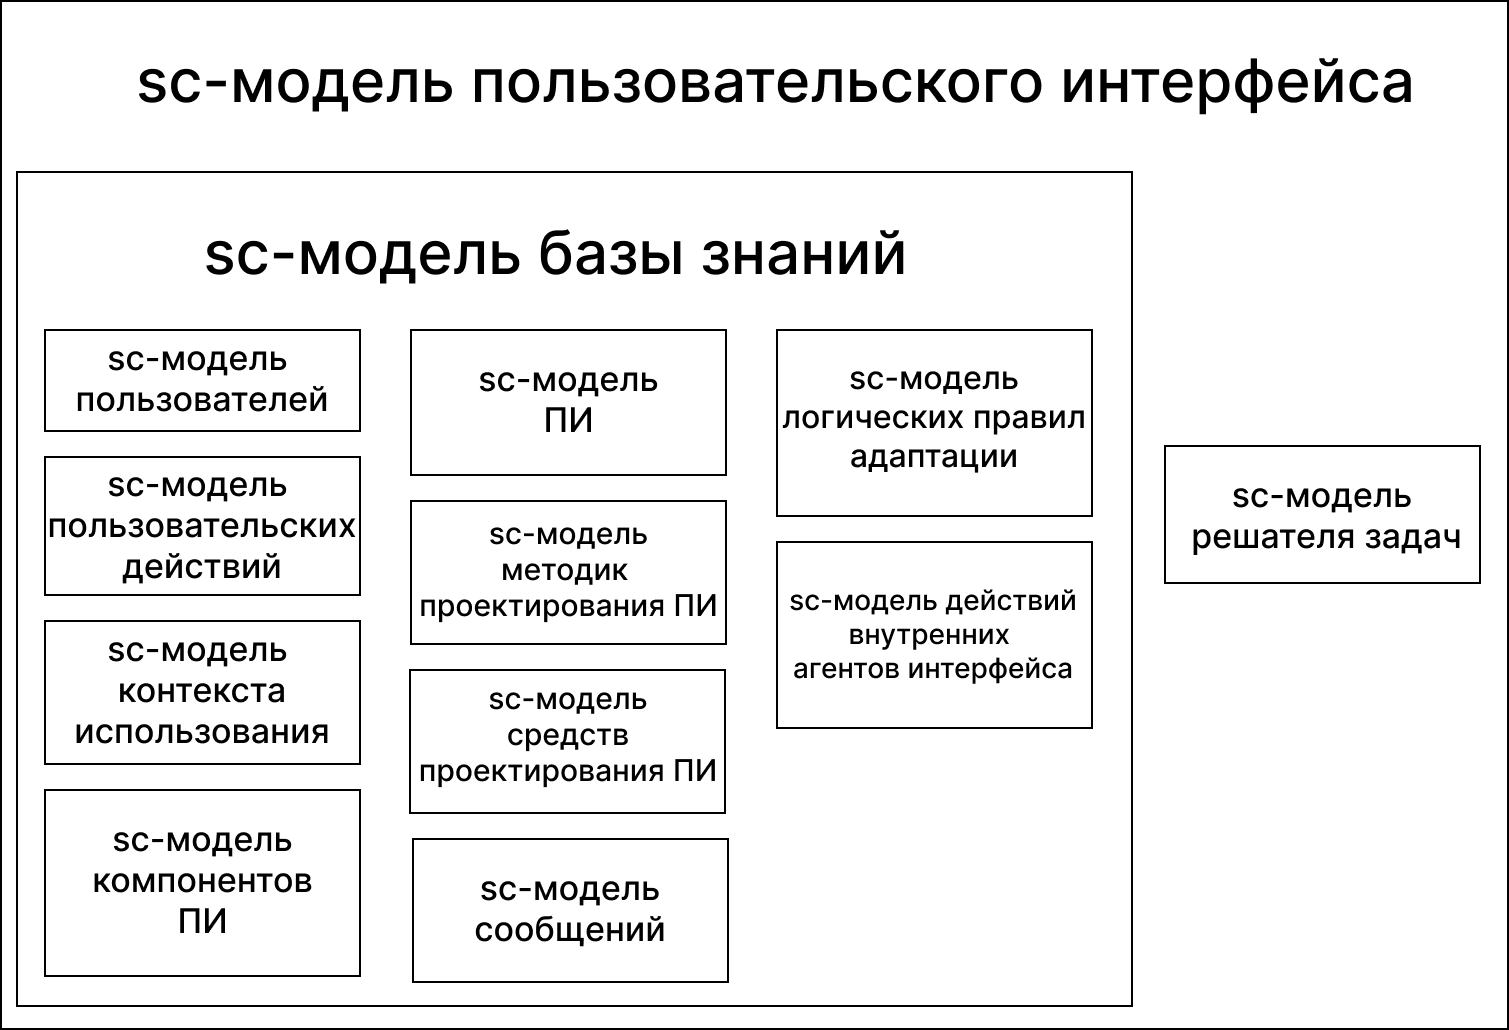
\includegraphics[scale=0.15]{images/part5/sc-model-ui.png}
\end{figure}

Таким образом, предлагаемая методика проектирования интерфейсов ostis-систем будет включать:
\begin{textitemize}
\item анализ пользователя, его задач и целей, а также контекста использования;
\item анализ требований к пользовательскому интерфейсу;
\item проектирование пользовательского интерфейса по умолчанию;
\item разработка пользовательского интерфейса;
\item анализ пользовательского интерфейса и его адаптации.
\end{textitemize}

Поскольку знания о конкретном этапе обычно находятся у разных экспертов, особенностью предлагаемого подхода является обязательное формализованное документирование знаний в унифицированном виде и применение на каждом из этапов компонентного подхода.

Для применения компонентного подхода предлагается использовать \textit{библиотеку многократно используемых компонентов} базы знаний, решателя задач и интерфейса.

\scnheader{Анализ пользователя, его задач и целей, а также контекста использования}

Результаты первого этапа, такие как: модель конкретного пользователя, его потребности и контекст использования системы (устройство, окружающая среда) должны быть формализованы в рамках соответствующих онтологий базы знаний интерфейса. 
При этом в процессе формализации по необходимости должны быть переиспользованы компоненты базы знаний из библиотеки многократно используемых компонентов, а новые компоненты могут пополнить эту же библиотеку.

\scnheader{Анализ требований к пользовательскому интерфейсу}

Результатом второго этапа являются конечные требования к интерфейсу, которые должны быть сформулированы относительно модели пользователя и его цели, а также относительно контекста использования.

Результаты должны быть также формализованы, а в процессе выполнения могут быть использованы существующие компонент базы знаний из библиотеки многократно используемых компонентов.

\scnheader{Проектирование пользовательского интерфейса по умолчанию}

В соответствии с требованиями к пользовательскому интерфейсу, строится модель адаптивного интеллектуального мультимодального пользовательского интерфейса, которая является результатом третьего этапа.

Такая модель будет включать в себя формализованную модель базы знаний и решателя задач.

При проектировании могут быть использованы компоненты интерфейса, базы знаний и решателя задач. 
Компоненты будут записаны в унифицированном виде, что позволит обеспечить их автоматическую совместимость.

\scnheader{Разработка пользовательского интерфейса}

Результатом четвертого этапа является реализация спроектированного пользовательского интерфейса. В данном случае следует использовать готовые компоненты интерфейса из библиотеки многократно используемых компонентов интерфейса.

\scnheader{Анализ пользовательского интерфейса и его адаптации}
На данном этапе используются готовые компоненты решателя задач.


Таким образом будет сформирована база знаний проектируемого интерфейса, которая автоматически может быть использована в качестве help-системы для пользователей, разработчиков и т.д.



\section{Логико-семантическая модель ostis-системы автоматизации проектирования интерфейсов ostis-систем}
\section{Многократно используемые компоненты интерфейсов ostis-систем}

%%%%%%%%%%%%%%%%%%%%%%%%% referenc.tex %%%%%%%%%%%%%%%%%%%%%%%%%%%%%%
% sample references
% %
% Use this file as a template for your own input.
%
%%%%%%%%%%%%%%%%%%%%%%%% Springer-Verlag %%%%%%%%%%%%%%%%%%%%%%%%%%
%
% BibTeX users please use
% \bibliographystyle{}
% \bibliography{}
%
\biblstarthook{In view of the parallel print and (chapter-wise) online publication of your book at \url{www.springerlink.com} it has been decided that -- as a genreral rule --  references should be sorted chapter-wise and placed at the end of the individual chapters. However, upon agreement with your contact at Springer you may list your references in a single seperate chapter at the end of your book. Deactivate the class option \texttt{sectrefs} and the \texttt{thebibliography} environment will be put out as a chapter of its own.\\\indent
References may be \textit{cited} in the text either by number (preferred) or by author/year.\footnote{Make sure that all references from the list are cited in the text. Those not cited should be moved to a separate \textit{Further Reading} section or chapter.} If the citatiion in the text is numbered, the reference list should be arranged in ascending order. If the citation in the text is author/year, the reference list should be \textit{sorted} alphabetically and if there are several works by the same author, the following order should be used:
\begin{enumerate}
\item all works by the author alone, ordered chronologically by year of publication
\item all works by the author with a coauthor, ordered alphabetically by coauthor
\item all works by the author with several coauthors, ordered chronologically by year of publication.
\end{enumerate}
The \textit{styling} of references\footnote{Always use the standard abbreviation of a journal's name according to the ISSN \textit{List of Title Word Abbreviations}, see \url{http://www.issn.org/en/node/344}} depends on the subject of your book:
\begin{itemize}
\item The \textit{two} recommended styles for references in books on \textit{mathematical, physical, statistical and computer sciences} are depicted in ~\cite{science-contrib, science-online, science-mono, science-journal, science-DOI} and ~\cite{phys-online, phys-mono, phys-journal, phys-DOI, phys-contrib}.
\item Examples of the most commonly used reference style in books on \textit{Psychology, Social Sciences} are~\cite{psysoc-mono, psysoc-online,psysoc-journal, psysoc-contrib, psysoc-DOI}.
\item Examples for references in books on \textit{Humanities, Linguistics, Philosophy} are~\cite{humlinphil-journal, humlinphil-contrib, humlinphil-mono, humlinphil-online, humlinphil-DOI}.
\item Examples of the basic Springer style used in publications on a wide range of subjects such as \textit{Computer Science, Economics, Engineering, Geosciences, Life Sciences, Medicine, Biomedicine} are ~\cite{basic-contrib, basic-online, basic-journal, basic-DOI, basic-mono}. 
\end{itemize}
}

\begin{thebibliography}{99.}%
% and use \bibitem to create references.
%
% Use the following syntax and markup for your references if 
% the subject of your book is from the field 
% "Mathematics, Physics, Statistics, Computer Science"
%
% Contribution 
\bibitem{science-contrib} Broy, M.: Software engineering --- from auxiliary to key technologies. In: Broy, M., Dener, E. (eds.) Software Pioneers, pp. 10-13. Springer, Heidelberg (2002)
%
% Online Document
\bibitem{science-online} Dod, J.: Effective substances. In: The Dictionary of Substances and Their Effects. Royal Society of Chemistry (1999) Available via DIALOG. \\
\url{http://www.rsc.org/dose/title of subordinate document. Cited 15 Jan 1999}
%
% Monograph
\bibitem{science-mono} Geddes, K.O., Czapor, S.R., Labahn, G.: Algorithms for Computer Algebra. Kluwer, Boston (1992) 
%
% Journal article
\bibitem{science-journal} Hamburger, C.: Quasimonotonicity, regularity and duality for nonlinear systems of partial differential equations. Ann. Mat. Pura. Appl. \textbf{169}, 321--354 (1995)
%
% Journal article by DOI
\bibitem{science-DOI} Slifka, M.K., Whitton, J.L.: Clinical implications of dysregulated cytokine production. J. Mol. Med. (2000) doi: 10.1007/s001090000086 
%
\bigskip

% Use the following (APS) syntax and markup for your references if 
% the subject of your book is from the field 
% "Mathematics, Physics, Statistics, Computer Science"
%
% Online Document
\bibitem{phys-online} J. Dod, in \textit{The Dictionary of Substances and Their Effects}, Royal Society of Chemistry. (Available via DIALOG, 1999), 
\url{http://www.rsc.org/dose/title of subordinate document. Cited 15 Jan 1999}
%
% Monograph
\bibitem{phys-mono} H. Ibach, H. L\"uth, \textit{Solid-State Physics}, 2nd edn. (Springer, New York, 1996), pp. 45-56 
%
% Journal article
\bibitem{phys-journal} S. Preuss, A. Demchuk Jr., M. Stuke, Appl. Phys. A \textbf{61}
%
% Journal article by DOI
\bibitem{phys-DOI} M.K. Slifka, J.L. Whitton, J. Mol. Med., doi: 10.1007/s001090000086
%
% Contribution 
\bibitem{phys-contrib} S.E. Smith, in \textit{Neuromuscular Junction}, ed. by E. Zaimis. Handbook of Experimental Pharmacology, vol 42 (Springer, Heidelberg, 1976), p. 593
%
\bigskip
%
% Use the following syntax and markup for your references if 
% the subject of your book is from the field 
% "Psychology, Social Sciences"
%
%
% Monograph
\bibitem{psysoc-mono} Calfee, R.~C., \& Valencia, R.~R. (1991). \textit{APA guide to preparing manuscripts for journal publication.} Washington, DC: American Psychological Association.
%
% Online Document
\bibitem{psysoc-online} Dod, J. (1999). Effective substances. In: The dictionary of substances and their effects. Royal Society of Chemistry. Available via DIALOG. \\
\url{http://www.rsc.org/dose/Effective substances.} Cited 15 Jan 1999.
%
% Journal article
\bibitem{psysoc-journal} Harris, M., Karper, E., Stacks, G., Hoffman, D., DeNiro, R., Cruz, P., et al. (2001). Writing labs and the Hollywood connection. \textit{J Film} Writing, 44(3), 213--245.
%
% Contribution 
\bibitem{psysoc-contrib} O'Neil, J.~M., \& Egan, J. (1992). Men's and women's gender role journeys: Metaphor for healing, transition, and transformation. In B.~R. Wainrig (Ed.), \textit{Gender issues across the life cycle} (pp. 107--123). New York: Springer.
%
% Journal article by DOI
\bibitem{psysoc-DOI}Kreger, M., Brindis, C.D., Manuel, D.M., Sassoubre, L. (2007). Lessons learned in systems change initiatives: benchmarks and indicators. \textit{American Journal of Community Psychology}, doi: 10.1007/s10464-007-9108-14.
%
%
% Use the following syntax and markup for your references if 
% the subject of your book is from the field 
% "Humanities, Linguistics, Philosophy"
%
\bigskip
%
% Journal article
\bibitem{humlinphil-journal} Alber John, Daniel C. O'Connell, and Sabine Kowal. 2002. Personal perspective in TV interviews. \textit{Pragmatics} 12:257--271
%
% Contribution 
\bibitem{humlinphil-contrib} Cameron, Deborah. 1997. Theoretical debates in feminist linguistics: Questions of sex and gender. In \textit{Gender and discourse}, ed. Ruth Wodak, 99--119. London: Sage Publications.
%
% Monograph
\bibitem{humlinphil-mono} Cameron, Deborah. 1985. \textit{Feminism and linguistic theory.} New York: St. Martin's Press.
%
% Online Document
\bibitem{humlinphil-online} Dod, Jake. 1999. Effective substances. In: The dictionary of substances and their effects. Royal Society of Chemistry. Available via DIALOG. \\
http://www.rsc.org/dose/title of subordinate document. Cited 15 Jan 1999
%
% Journal article by DOI
\bibitem{humlinphil-DOI} Suleiman, Camelia, Daniel C. O'Connell, and Sabine Kowal. 2002. `If you and I, if we, in this later day, lose that sacred fire...': Perspective in political interviews. \textit{Journal of Psycholinguistic Research}. doi: 10.1023/A:1015592129296.
%
%
%
\bigskip
%
%
% Use the following syntax and markup for your references if 
% the subject of your book is from the field 
% "Computer Science, Economics, Engineering, Geosciences, Life Sciences"
%
%
% Contribution 
\bibitem{basic-contrib} Brown B, Aaron M (2001) The politics of nature. In: Smith J (ed) The rise of modern genomics, 3rd edn. Wiley, New York 
%
% Online Document
\bibitem{basic-online} Dod J (1999) Effective Substances. In: The dictionary of substances and their effects. Royal Society of Chemistry. Available via DIALOG. \\
\url{http://www.rsc.org/dose/title of subordinate document. Cited 15 Jan 1999}
%
% Journal article by DOI
\bibitem{basic-DOI} Slifka MK, Whitton JL (2000) Clinical implications of dysregulated cytokine production. J Mol Med, doi: 10.1007/s001090000086
%
% Journal article
\bibitem{basic-journal} Smith J, Jones M Jr, Houghton L et al (1999) Future of health insurance. N Engl J Med 965:325--329
%
% Monograph
\bibitem{basic-mono} South J, Blass B (2001) The future of modern genomics. Blackwell, London 
%
\end{thebibliography}

